\documentclass[14pt]{extreport}
\usepackage[utf8]{inputenc}
\usepackage[russian]{babel}
\usepackage[top=20pt,bottom=70pt,left=40pt,right=40pt]{geometry}
\usepackage{amssymb}
\usepackage{amsmath}
\usepackage{graphicx}
\usepackage[nottoc]{tocbibind}
\renewcommand*\rmdefault{cmr}

\begin{document}
	\begin{titlepage}
		\begin{center}  
			\large{Московский государственный университет имени М.В. Ломоносова\\
			Факультет вычислительной математики и кибернетики}\\
		\end{center}
		\begin{center}
			\vspace{160pt}
			\LARGE{\textbf{Формальные языки и автоматы\\}}
			\LARGE{\textbf{Методичка для сдающих и пересдающих}}
			\vspace{320pt}
		\end{center}
		\begin{center}
			\large{Может, зайдет кому-нибудь}
		\end{center}
	\end{titlepage}
	\newpage
	\tableofcontents
	\newpage
	\chapter*{Предисловие}
		Однажды я сдавал формалки. Не самый приятный опыт в моей жизни. Когда я ждал результатов,
		я сказал, что если не сдам, напишу методичку по этому чудесному предмету.\\
		\\
		Как несложно догадаться, я тогда не сдал.
		\\\\
		По формалкам уже есть отличное руководство в виде решений задач от Тани (не знаю, кто это,
		но если бы ее не было, статистика сдаваемости была бы гораздо хуже, я уверен, Таня,
		спасибо, что ты есть), и казалось
		бы - зачем я это делаю?\\
		Ну во-первых, я сказал, что напишу.\\
		Во-вторых, это довольно знатный способ подготовки к пересдаче, который потенциально
		поможет каким-нибудь людям после меня.\\
		В-третьих, наверное, есть смысл восполнить пробел в нормальном "печатном" пособии по
		формальным языкам. Ахо Ульмана я не читал (а он, может быть, и норм), но\ "Теорию
		Построения Комплияторов"\ читать совершенно невозможно.
		\\\\
		В этой методичке я в меру своих возможностей постараюсь не только подробно
		расписать решения различных задач (это уже есть у Тани), но и более-менее человеческим
		языком расписать, как применяемые алгоритмы работают (потому что выучить алгоритм, если
		есть примерное понимание работы, гораздо проще)
		\\\\
		За кривой русский язык извиняйте - я ЕГЭ сдал на 30 баллов.
	\newpage
	
	\chapter{Немного теормина}
	Недетерменированный конечный автомат - НКА
	\newpage
	
	\chapter{НКА по РВ}
	\section{Алгоритм}
	Построение НКА по РВ делается по определенным правилам\\
	Каждое РВ можно разбить на подвыражения, а для простейших подвыражений автомат строится
	довольно просто\\
	На рисунке далее\\
	1. Е-переход\\
	2. Переход по символу $a$\\
	3. Переход по $a|b$ ($a$ или $b$)\\
	4. Переход по $ab$ (сначала $a$, потом $b$)\\
	5. Переход по $a*$ (сколько угодно символов $a$, в т.ч. 0)\\
	Справа от простейших НКА нарисованы общие НКА, когда переход совершается
	по некоторому РВ, где $r$ - РВ, а $M(r)$ - НКА, построенный по нему.\\
	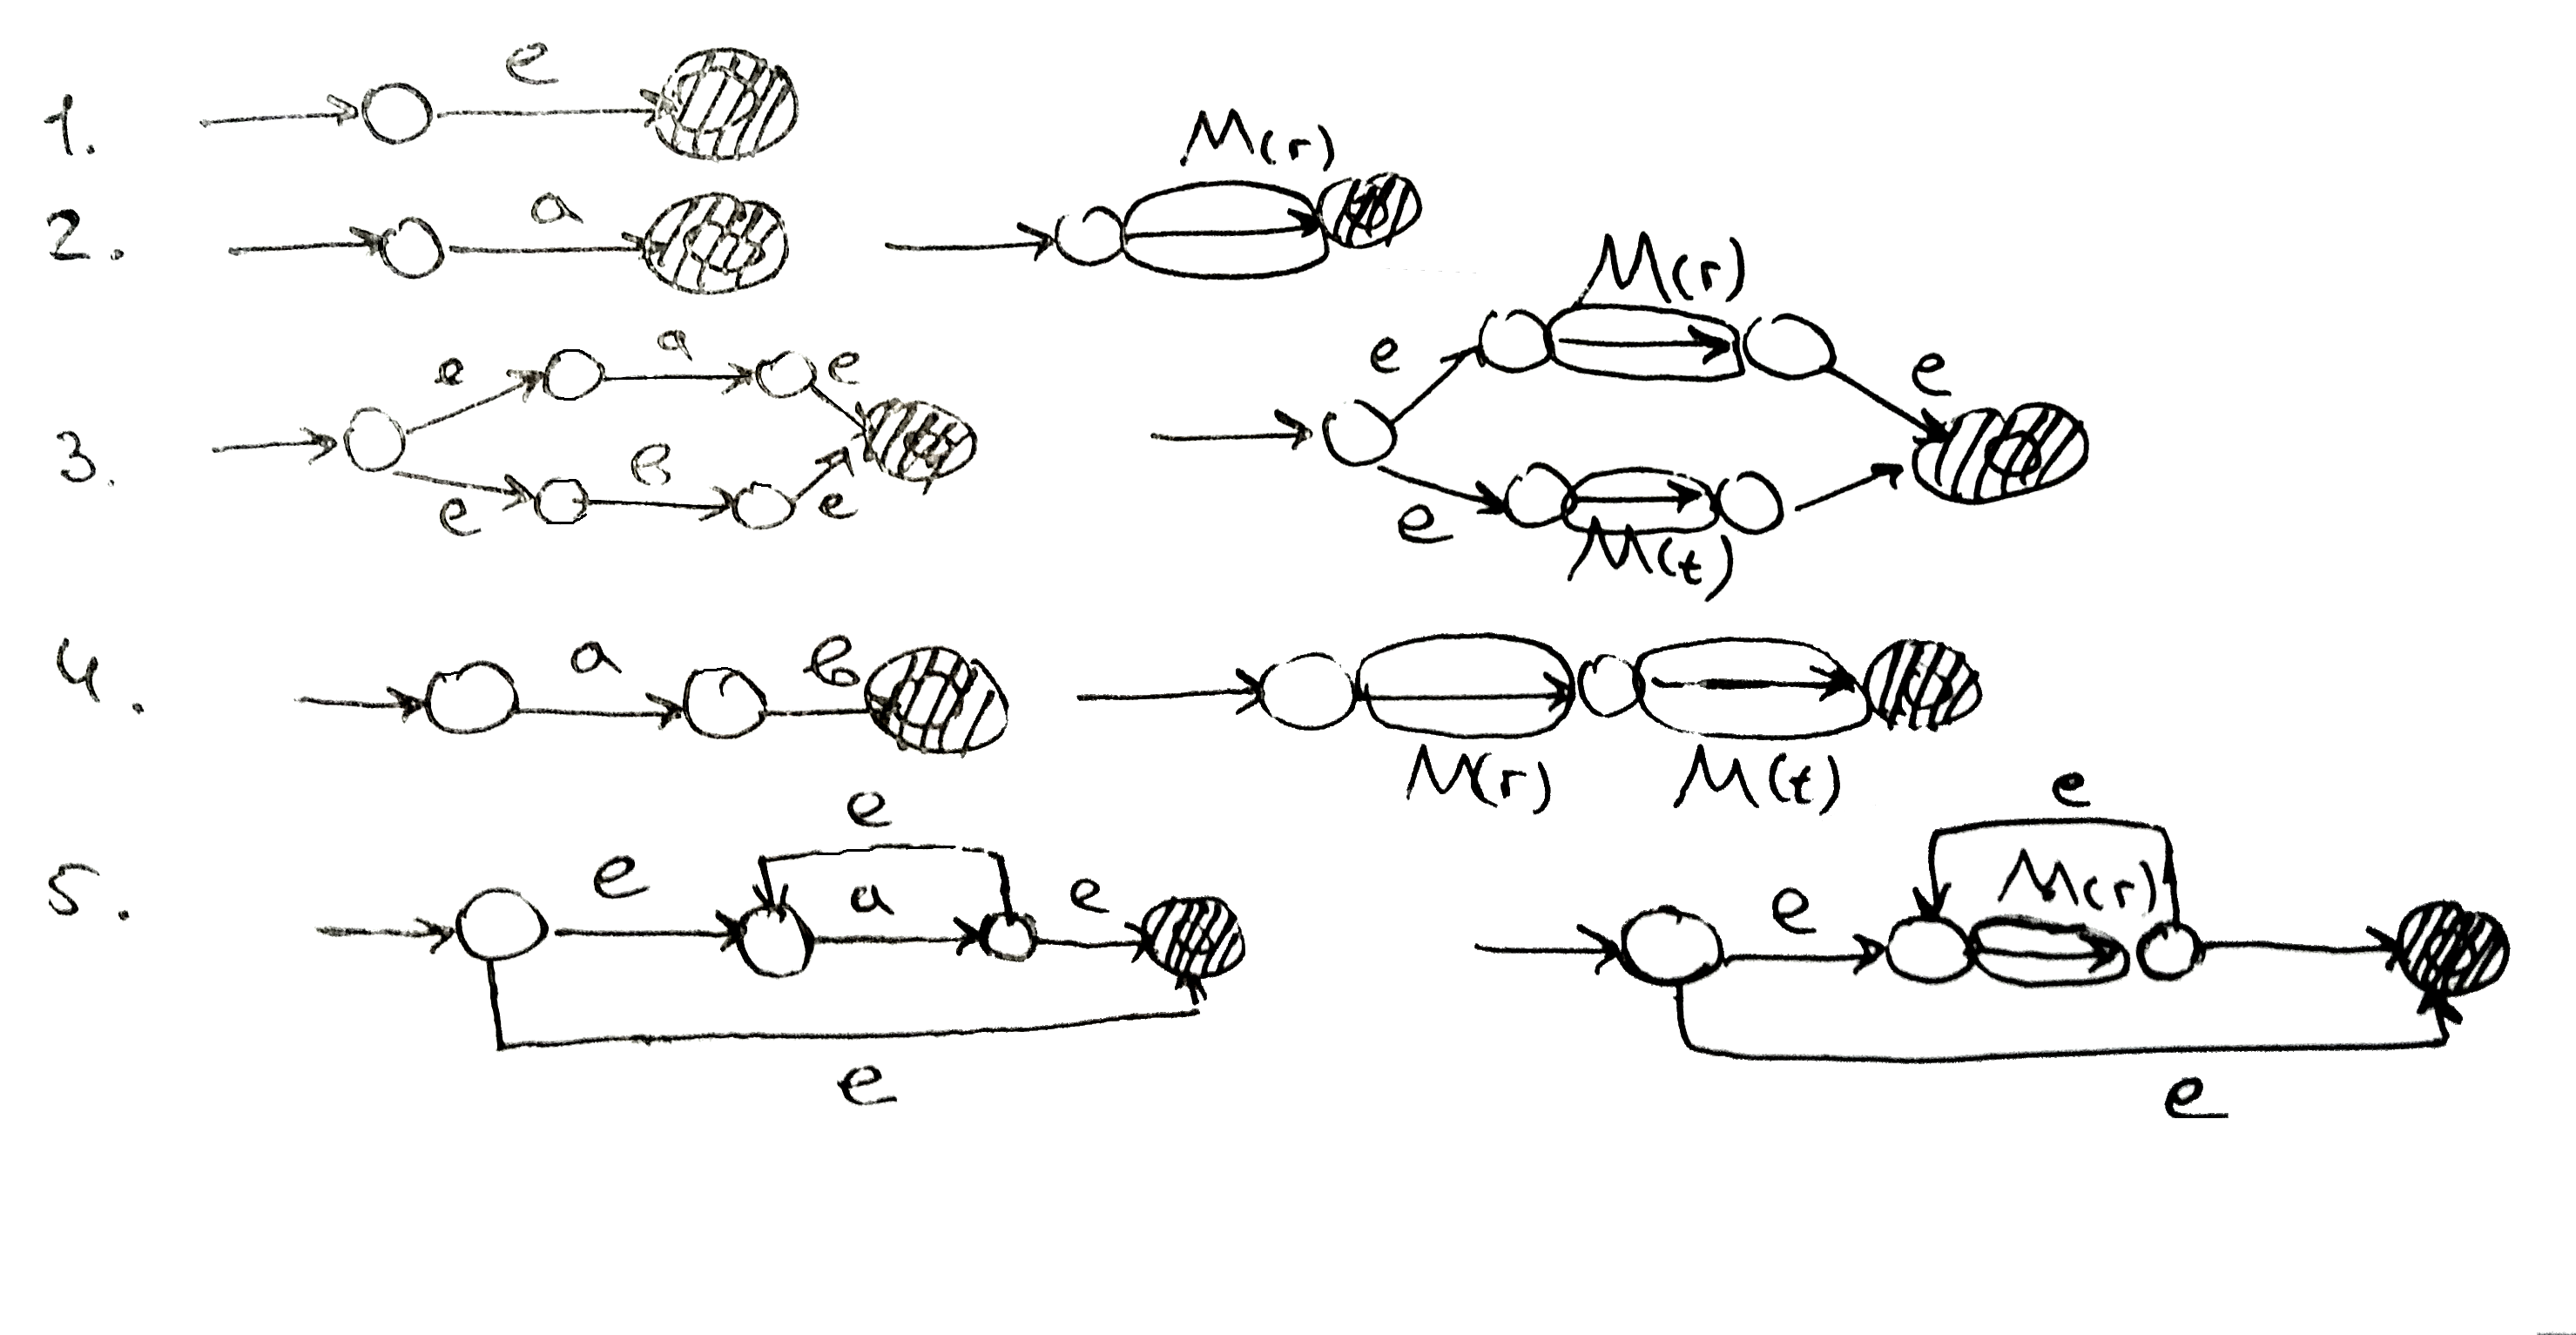
\includegraphics[scale=0.13]{data/pic1_1.png}\\\\\\\\
	На рисунке изображено построение НКА для РВ $b(a|ba)*|aab$\\
	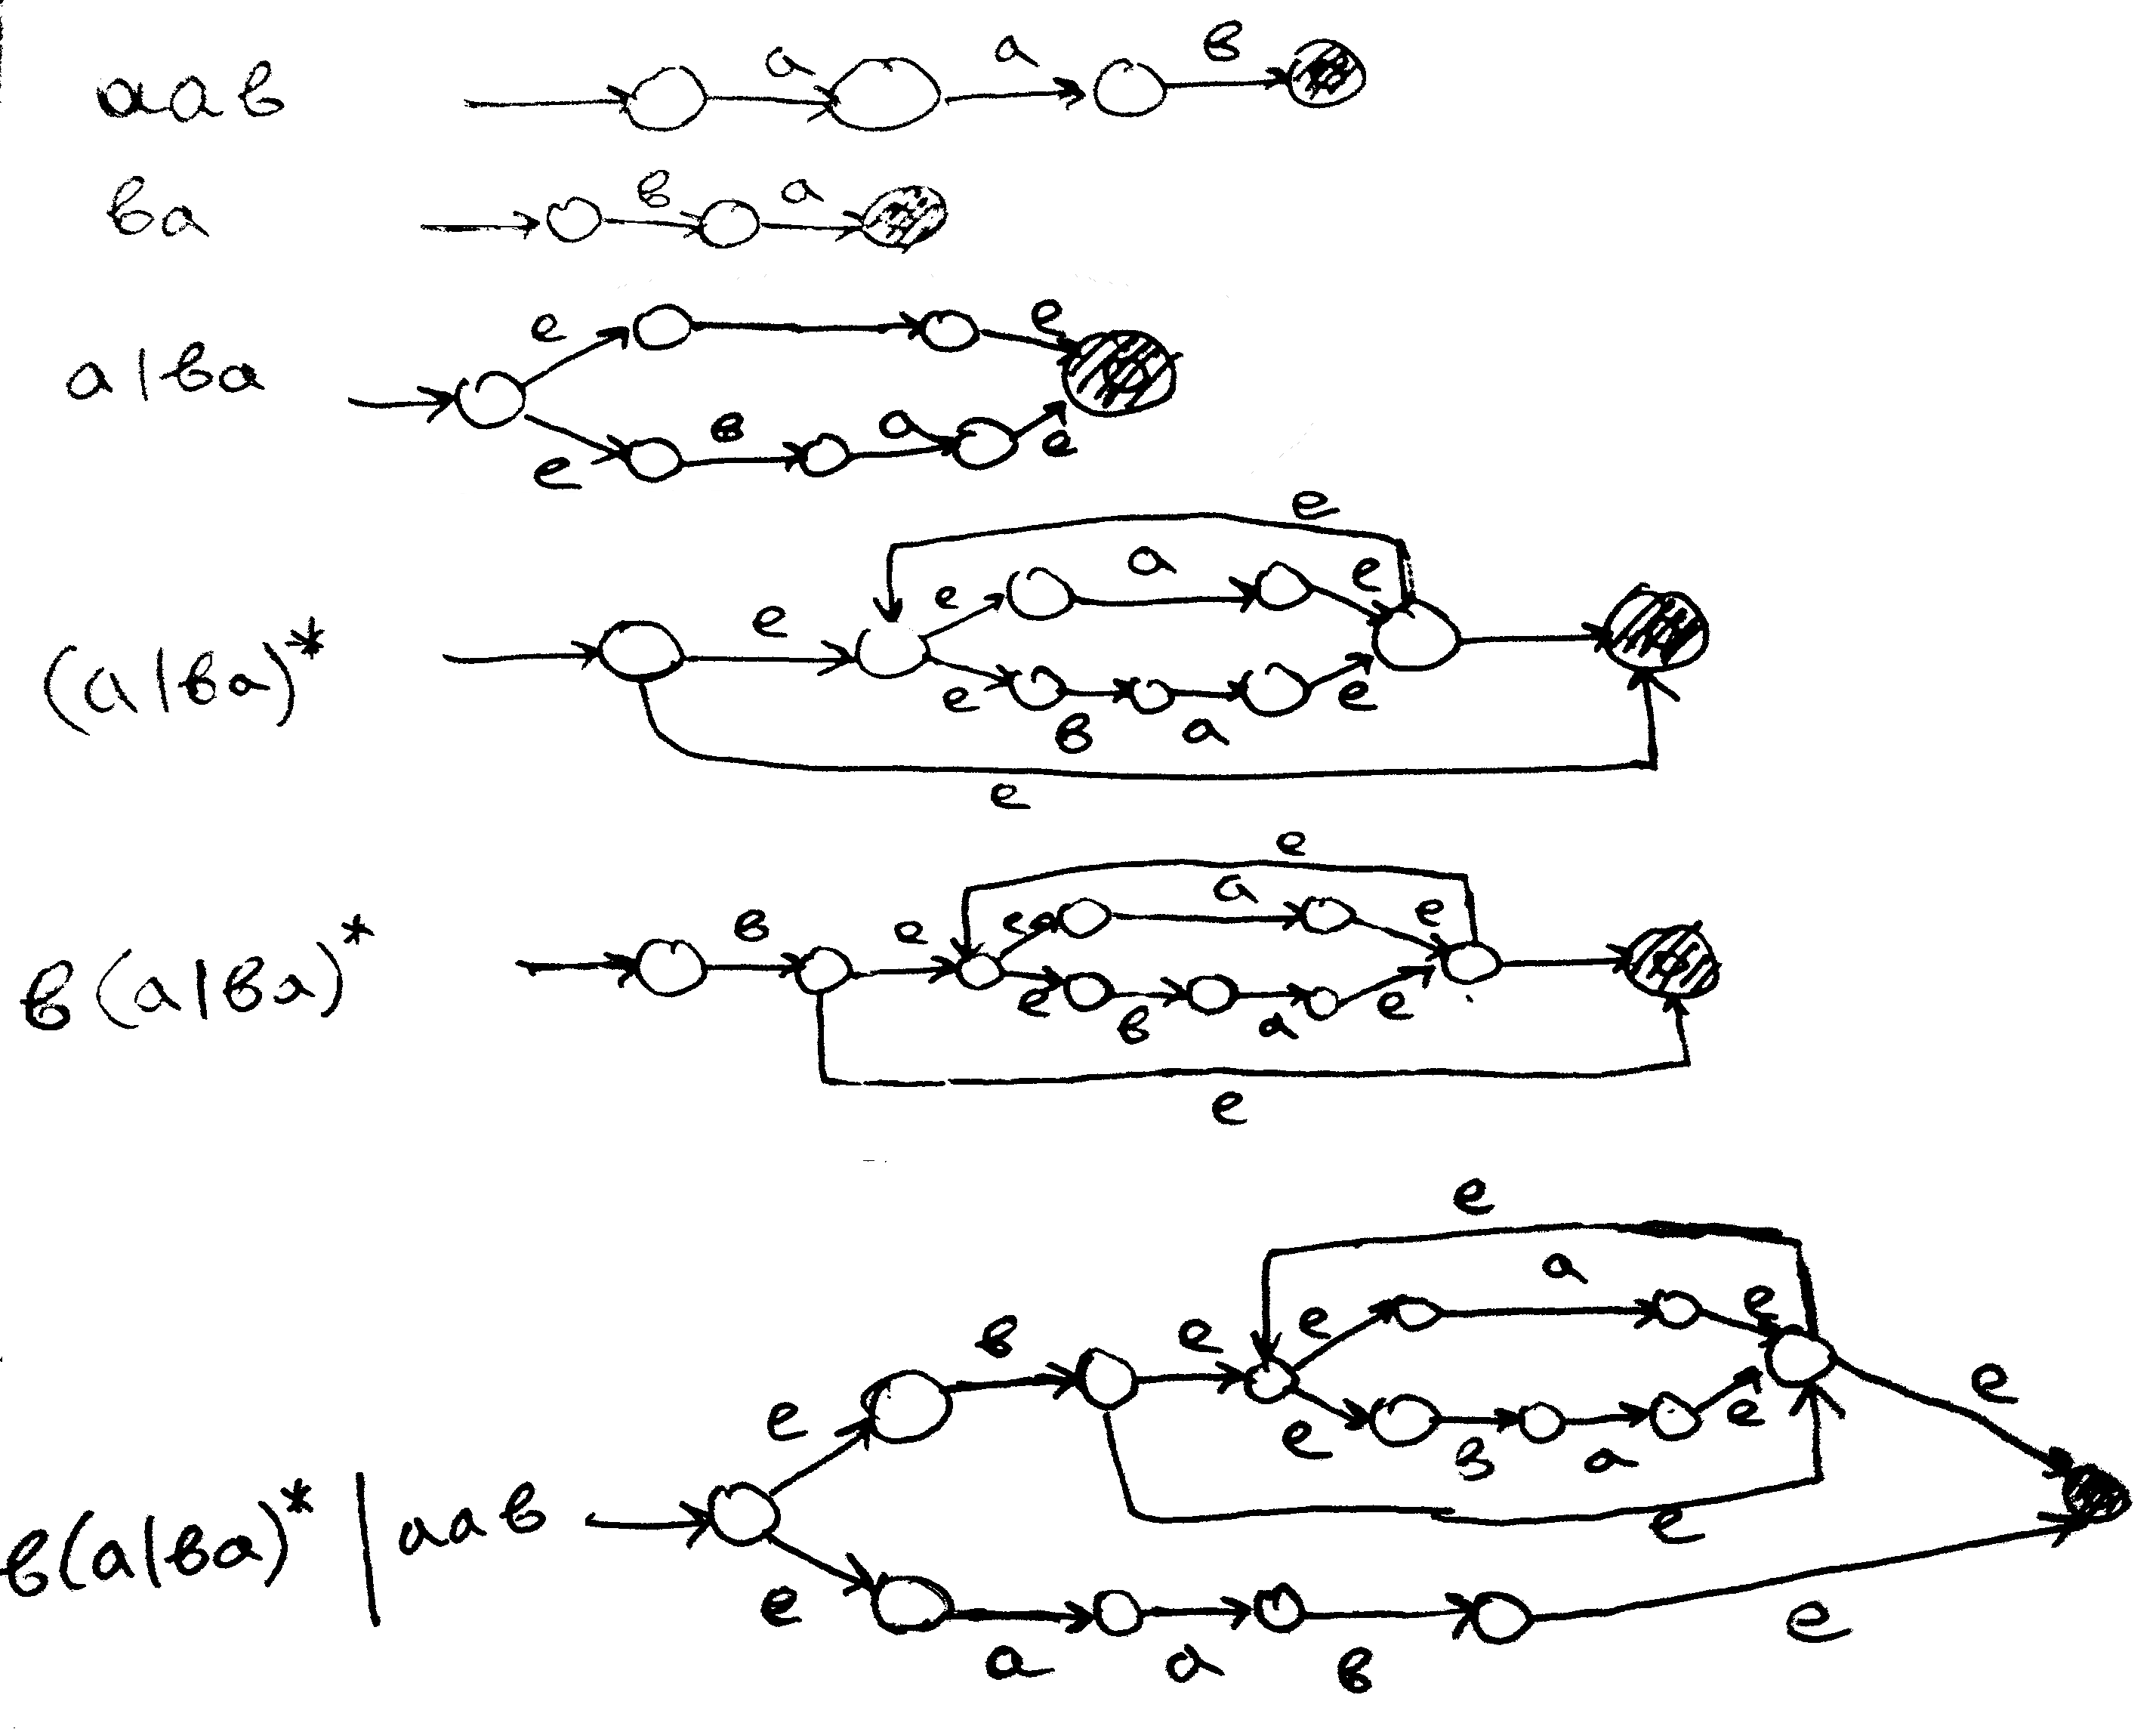
\includegraphics[scale=0.15]{data/pic1_2.png}\\
	\section{Почему это работает}
	Правильность таких построений довольно очевидна, но если не верится, можно походить по
	полученным НКА по дугам и убедиться, что ничего кроме того, что описано в РВ, по ним
	составить нельзя.
	\newpage
	
	\chapter{ДКА по НКА}
	Глядя на НКА, полученные по РВ может показаться, что там слишком много лишних e-переходов,
	и они бесят. Также НКА это вам не ДКА: есть неопределенности которые бесят (хотя процесс
	детерминирования бесит больше). В любом случае существует алгоритм, позволяющий из большого,
	но красивого НКА получить маленький и очень некрасивый ДКА.
	\section{Алгоритм}
	Введем некоторые обозначения:\\\\
	1. $e$-$closure(R)$ (эпсилон-замыкание состояния R) - множество состояний, в которые можно
	попасть из состояния $R$ по символу $e$. Стоит отметить, что "скачков"
	может быть больше одного,
	то есть, если в состояние $Q$ можно попасть из $P$ по $e$, а из $Q$ можно по $e$ попасть в $R$,
	то $R \in e$-$closure(Q)$. На языке умных людей это называется транзитивностью, но я тут не
	сложными словами щеголять пришел.\\\\
	2. $move(R, a)$ (достижимые из $R$ по $a$) - множество состояний, в которые можно попасть из
	состояния $R$ по символу $a$. (тут скачок должен быть только один)\\\\
	В качестве примера рассмотрим уродца из предыдущей главы:\\ $b(a|ba)*|aab$
	\newpage
	1. Для начала все состояния надо пронумеровать\\
	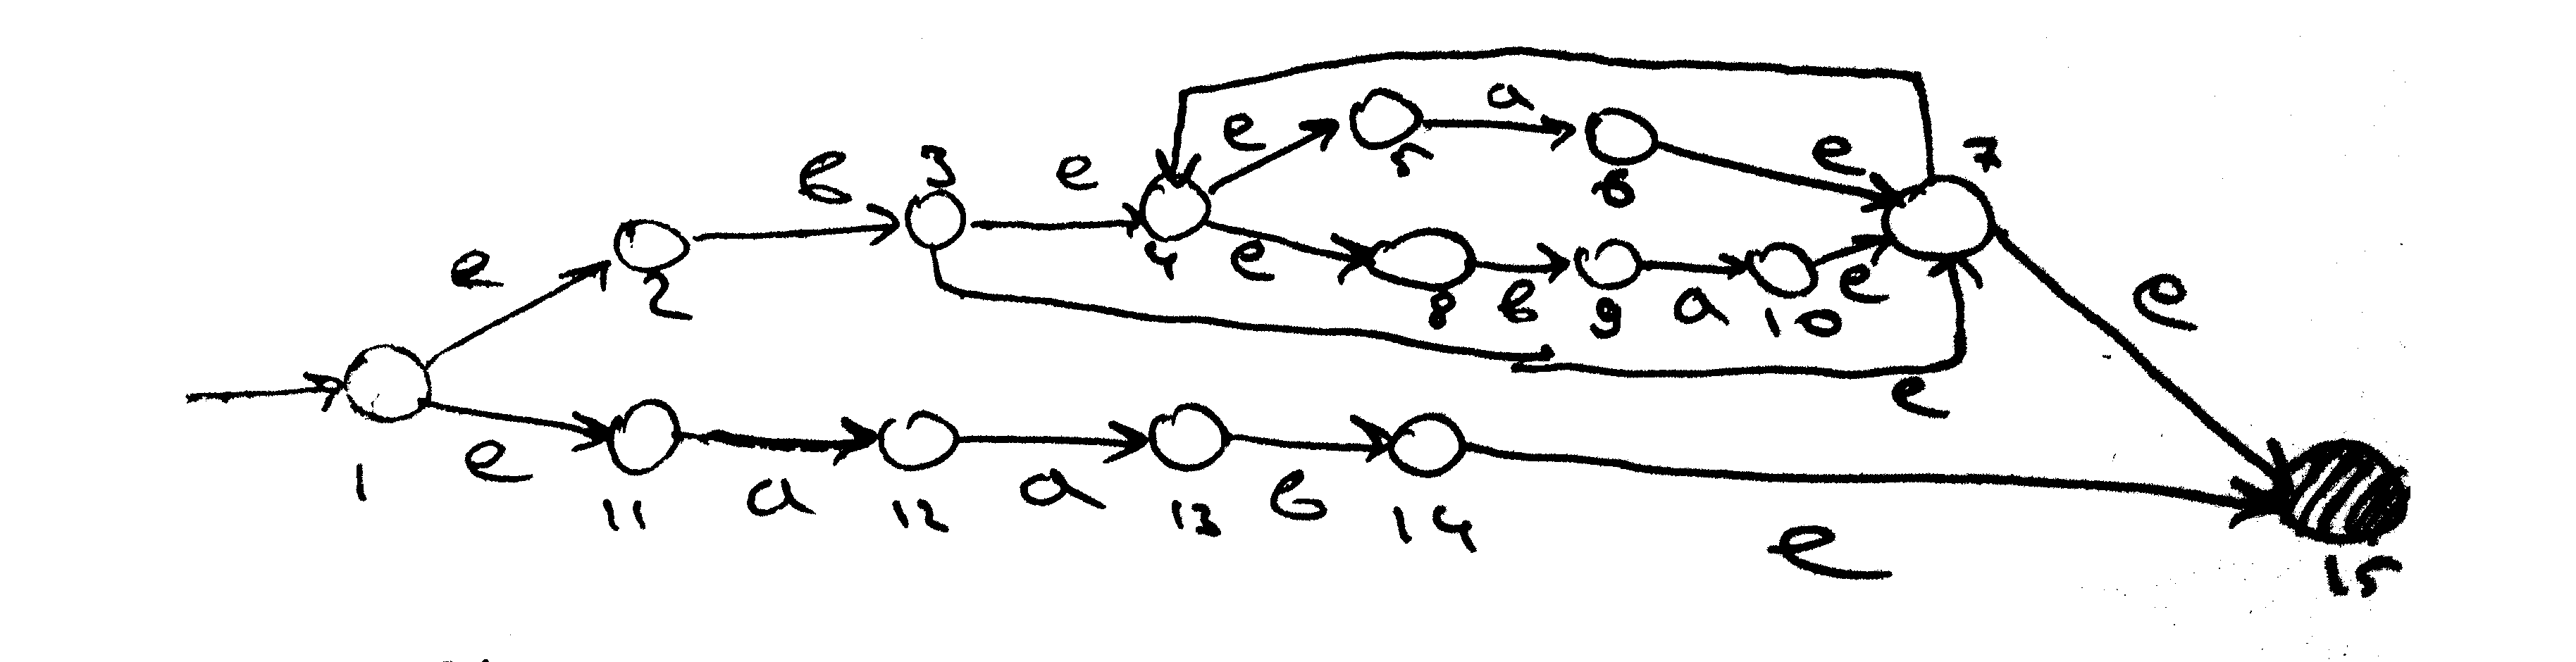
\includegraphics[scale=0.13]{data/pic2_1.png}\\
	На самом деле нумеровать их необязательно, главное дать им такие обозначения, чтобы
	вы сами могли отличить одно состояние от другого (ну и чтобы проверяющий экзаменатор не
	охерел, поэтому арабская вязь, наверное, не лучшее решение) - тут есть простор для фантазии,
	но на мой взгляд цифры вполне удобны (хотя между ними и приходится ставить запятые,
	если выписывать их в ряд).\\
	Далее мы начинаем описывать новый автомат с новыми состояниями - тут уже традиционно
	используют заглавные латинские буквы. Каждое новое состояние описывается множеством 
	старых состояний из первого автомата.\\\\
	2. В качестве начального состояния нового ДКА берут $A=e$-$closure(1)$, в нашем случае
	это $A=\{1, 2, 11\}$.\\\\
	3. Далее формируются следующие правила переходов:\\
	$D(A, a) = move(A, a)+e$-$closure(move(A, a))$\\
	$D(A, b) = move(A, b)+e$-$closure(move(A, b))$\\
	И т.д.\\\\
	Пусть вышло так, что есть состояние $Q$, из которого по символу $b$ мы переходим в состояние,
	описываемое множеством $\{1, 2, 3, 4, 6, 8, 12, 23\}$. При этом, если у такого множества уже
	есть имя, например $W$, то это попросту значит, что $D(Q, b)=W$. Если такого множества раньше
	не встречалось, то оно добавляется в таблицу состояний нового ДКА.\\
	Звучит сложно и скучно, поэтому лучше посмотреть на живой пример.\\
	$A=\{1, 2, 11\};$\\
	$move(A, a) = move(1, a)+move(2, a)+move(11,a);$\\
	$move(A,a)=\{\}+\{\}+\{12\}=\{12\};$\\
	$e$-$closure(move(A, a))=\{\};$\\
	$D(A, a) = move(A, a)+e$-$closure(move(A, a))=\{12\}+\{\}=\{12\};$\\
	Состояния $\{12\}$ у нас еще не было, поэтому добавим его в таблицу состояний и назовем его
	$B$.\\
	Проделаем аналогичные выкладки для символа $b$.\\
	$move(A, b) = move(1, b)+move(2, b)+move(11,b);$\\
	$move(A, b) = \{\}+\{3\}+\{\}=\{3\};$\\
	$e$-$closure(move(A, b))=\{4, 5, 7, 8, 15\};$\\
	$D(A, b) = move(A, b)+e$-$closure(move(A, b))=\{3\}+\{4, 5, 7, 8, 15\}=
	\{3, 4, 5, 7, 8, 15\};$\\
	Состояния $\{3, 4, 5, 7, 8, 15\}$ у нас тоже еще не было, поэтому запишем его в таблицу
	состояний ДКА.\\
	Подобные вычисления надо проводить для каждого символа в алфавите, для каждого нового
	состояния в таблице до тех пор, пока все старые состояния не будут описаны.\\
	С виду может показать, что это очень много писанины, но на деле все эти преобразования
	делаются в уме и единственное, что нужно реально выписывать, это таблицу состояний.\\
	Привожу финальную таблицу переходов для НКА из предыдущей главы.\\
		\begin{tabular}{lcc}
			 & $a$ & $b$ \\
			$A\{1, 2, 11\}$ & $B$ & $C$ \\
			$B\{12\}$ & $D$ & x \\
			$*C\{3, 4, 5, 7, 8, 15\}$ & $F$ & $G$ \\
			$D\{13\}$ & x & $E$ \\
			$*E\{14, 15\}$ & x & x \\
			$*F\{4, 5, 6, 7, 8, 15\}$ & $F$ & $G$ \\
			$G\{9\}$ & $H$ & x \\
			$*H\{4, 5, 7, 8, 10, 15\}$ & $F$ & $G$ \\	
		\end{tabular}\\\\
	Внимательный читатель заметит, что некоторые состояния отмечены звездочками и
	спросит, что это. Отвечаю: звездочками помечены конечные состояния. И это следующее
	правило алгоритма построения:\\\\
	4. Конечными состояниями нового ДКА помечаются такие состояния, которые содержат в себе
	конечное состояние старого НКА.\\
	В данном случае старым конечным состоянием является 15, поэтому все состояния, имеющие в себе
	15 становятся конечными.\\
	На рисунке изображен полученный ДКА.\\
	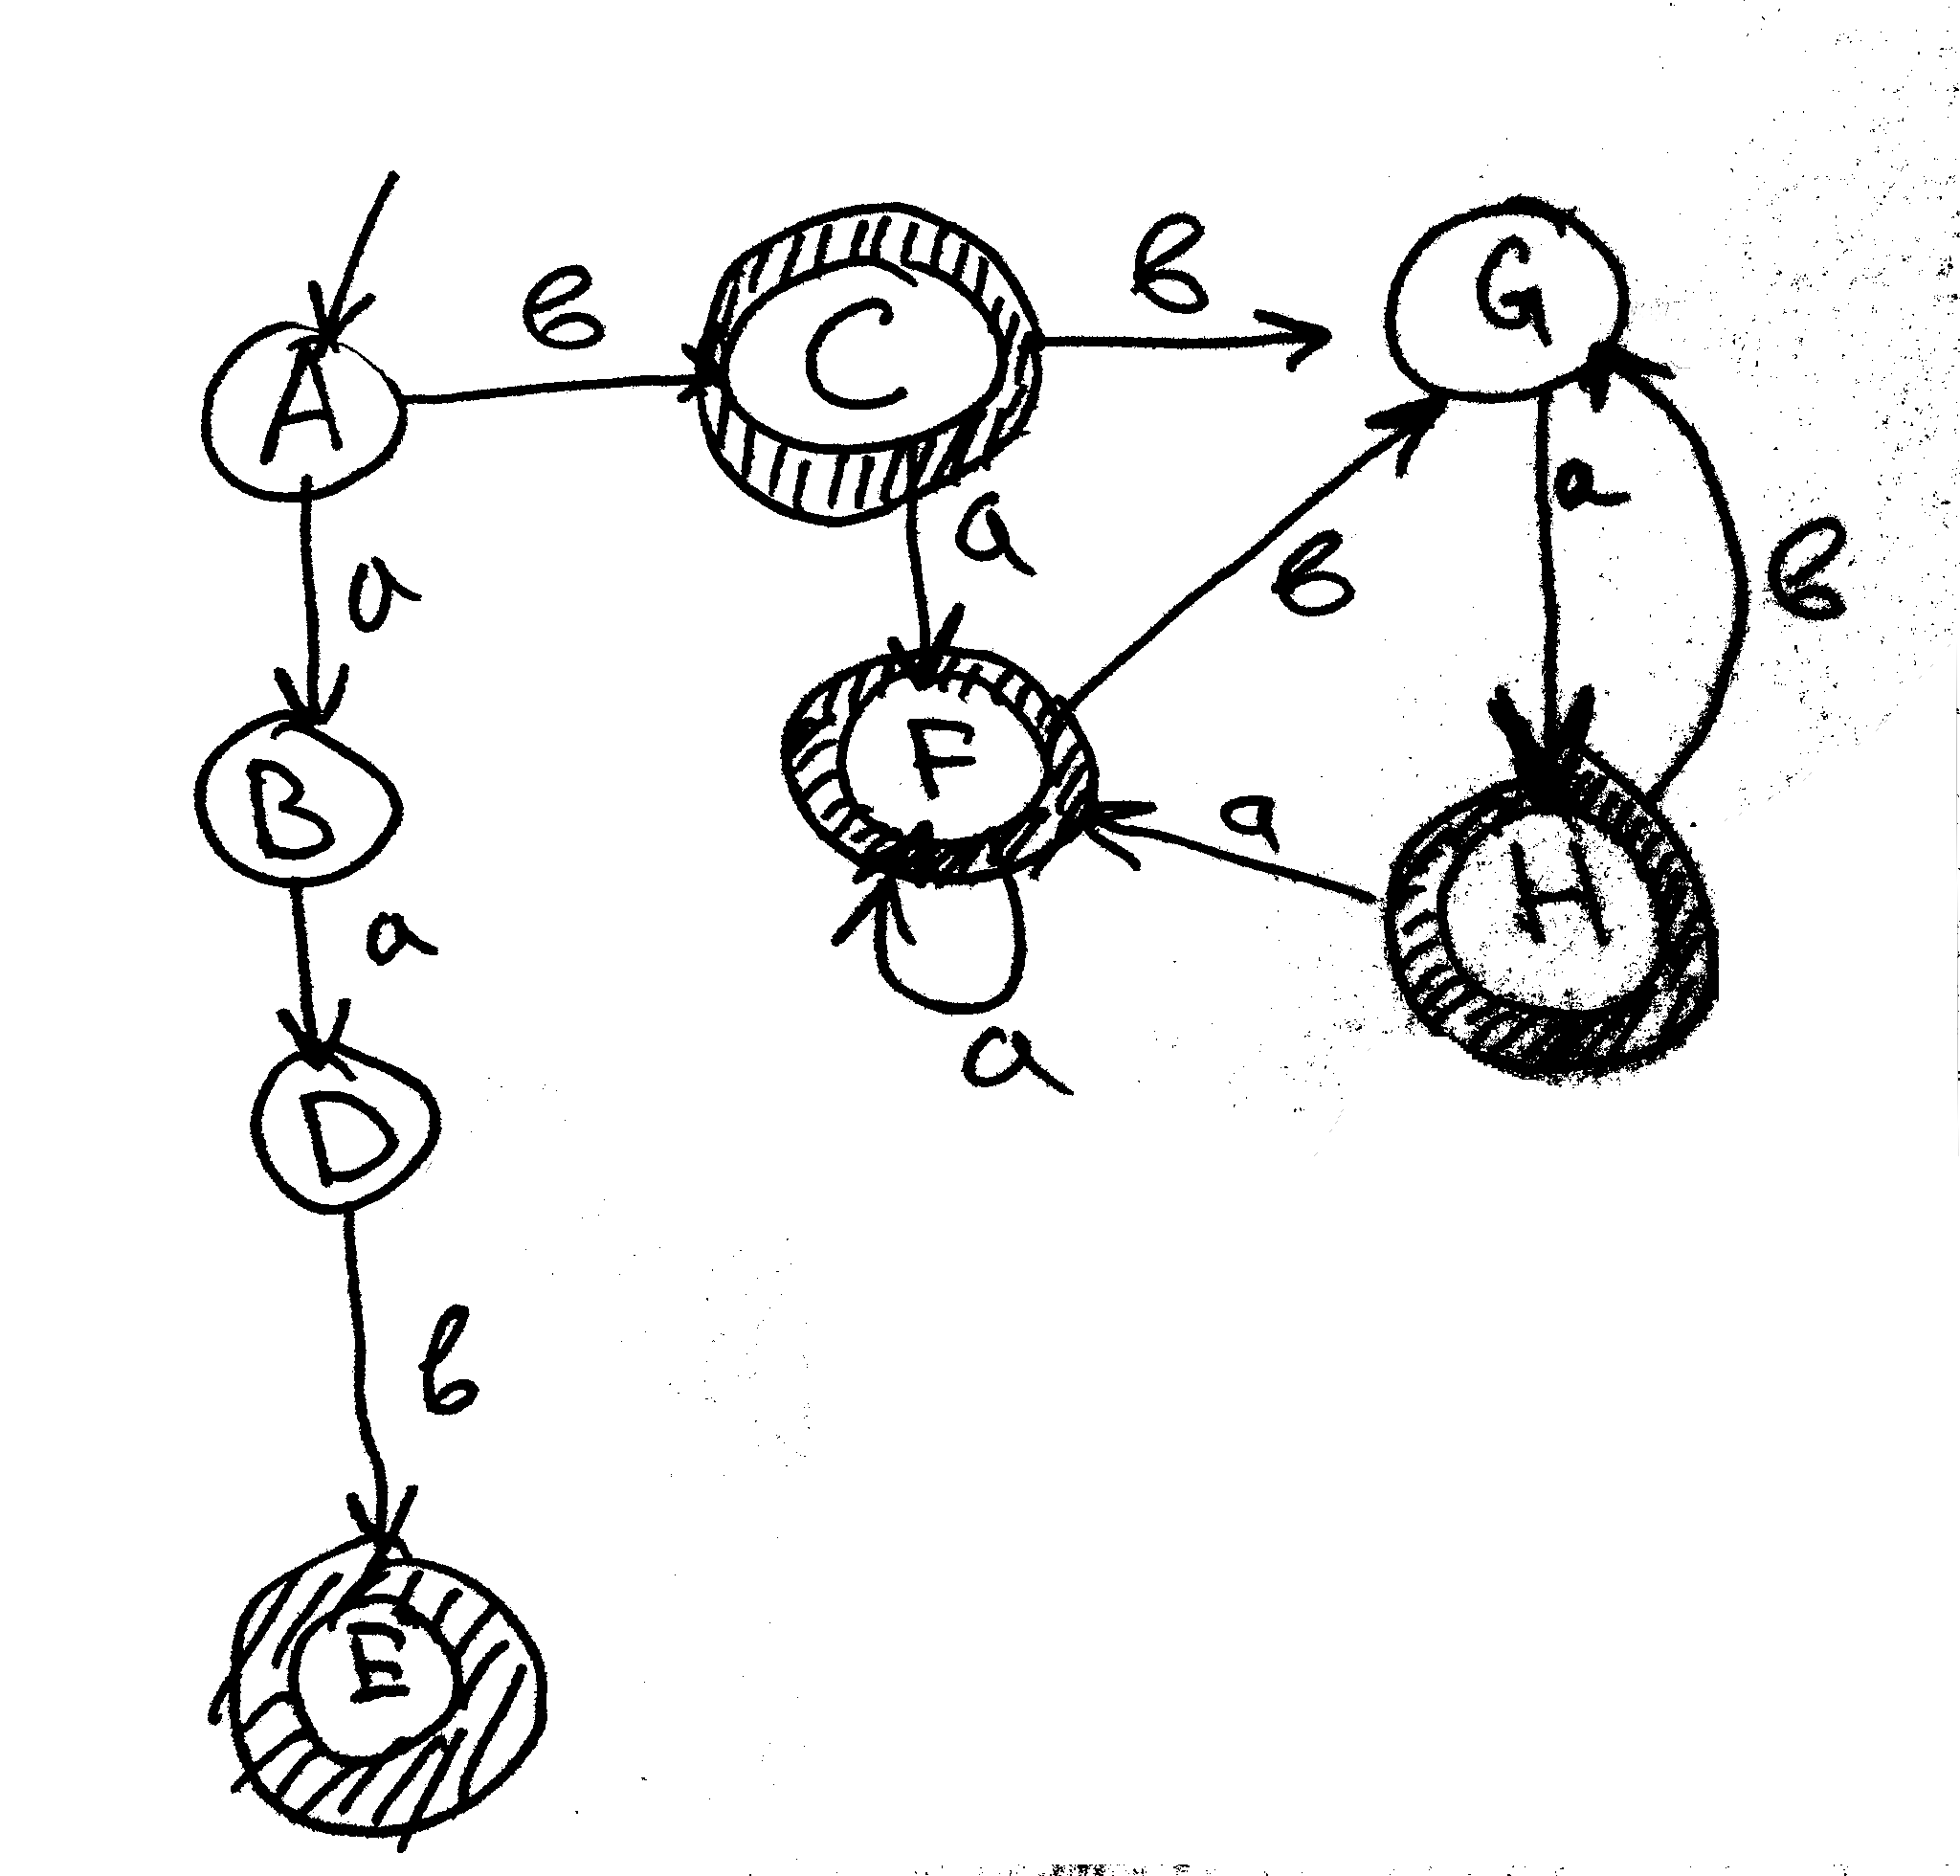
\includegraphics[scale=0.11]{data/pic2_2.png}\\
	\section{Почему это работает}
	Работа алгоритма строится на двух мыслях:\\
	1. Если из одного состояния по $e$ можно перейти в несколько других,
	то зачем нам эти другие состояния, если по сути состояние одно, просто
	разибитое на несколько частей? (незачем)\\
	Грубо говоря, мы стягиваем за $e$-дуги много состояний в одно, как за веревки.\\
	2. Если после стягиваний состояний, две дуги, раньше шедшие в два разных состояния,
	теперь идут в одно стянутое, то действительно ли между этими дугами есть разница? (нет)\\
	\newpage
	\chapter{ДКА по РВ}
	Допустим, что у нас есть РВ, которое необходимо преобразовать в ДКА. И казалось бы, уже есть
	целых 2 алгоритма, с помощью которых это можно сделать: сначала строим НКА, потом по нему же
	ДКА. Но есть более быстрый алгоритм прямого перевода.
	\section{Алгоритм}
	Для начала возьмем все то же РВ из первой главы $b(a|ba)*|aab$\\
	1. Строим расширение РВ: просто дописываем в конце символ конца, как бы странно
	это не звучало. Получаем $(b(a|ba)*|aab)\#$\\\\
	2. Нумеруем все буквы в нашем РВ (в том числе и символ конца)\\
	$(b(a|ba)*|aab)\#$\\
	\hspace*{5pt}$1\ 2\ 34\ \ \ \ \ 567\ 8$\\\\
	\newpage
	3. Строим дерево РВ (обязательно помним про приоритеты операций)\\
	Также на рисунке по бокам от каждого символа стоит его номер в РВ, чуть позже
	будет понятно, зачем.\\\\
	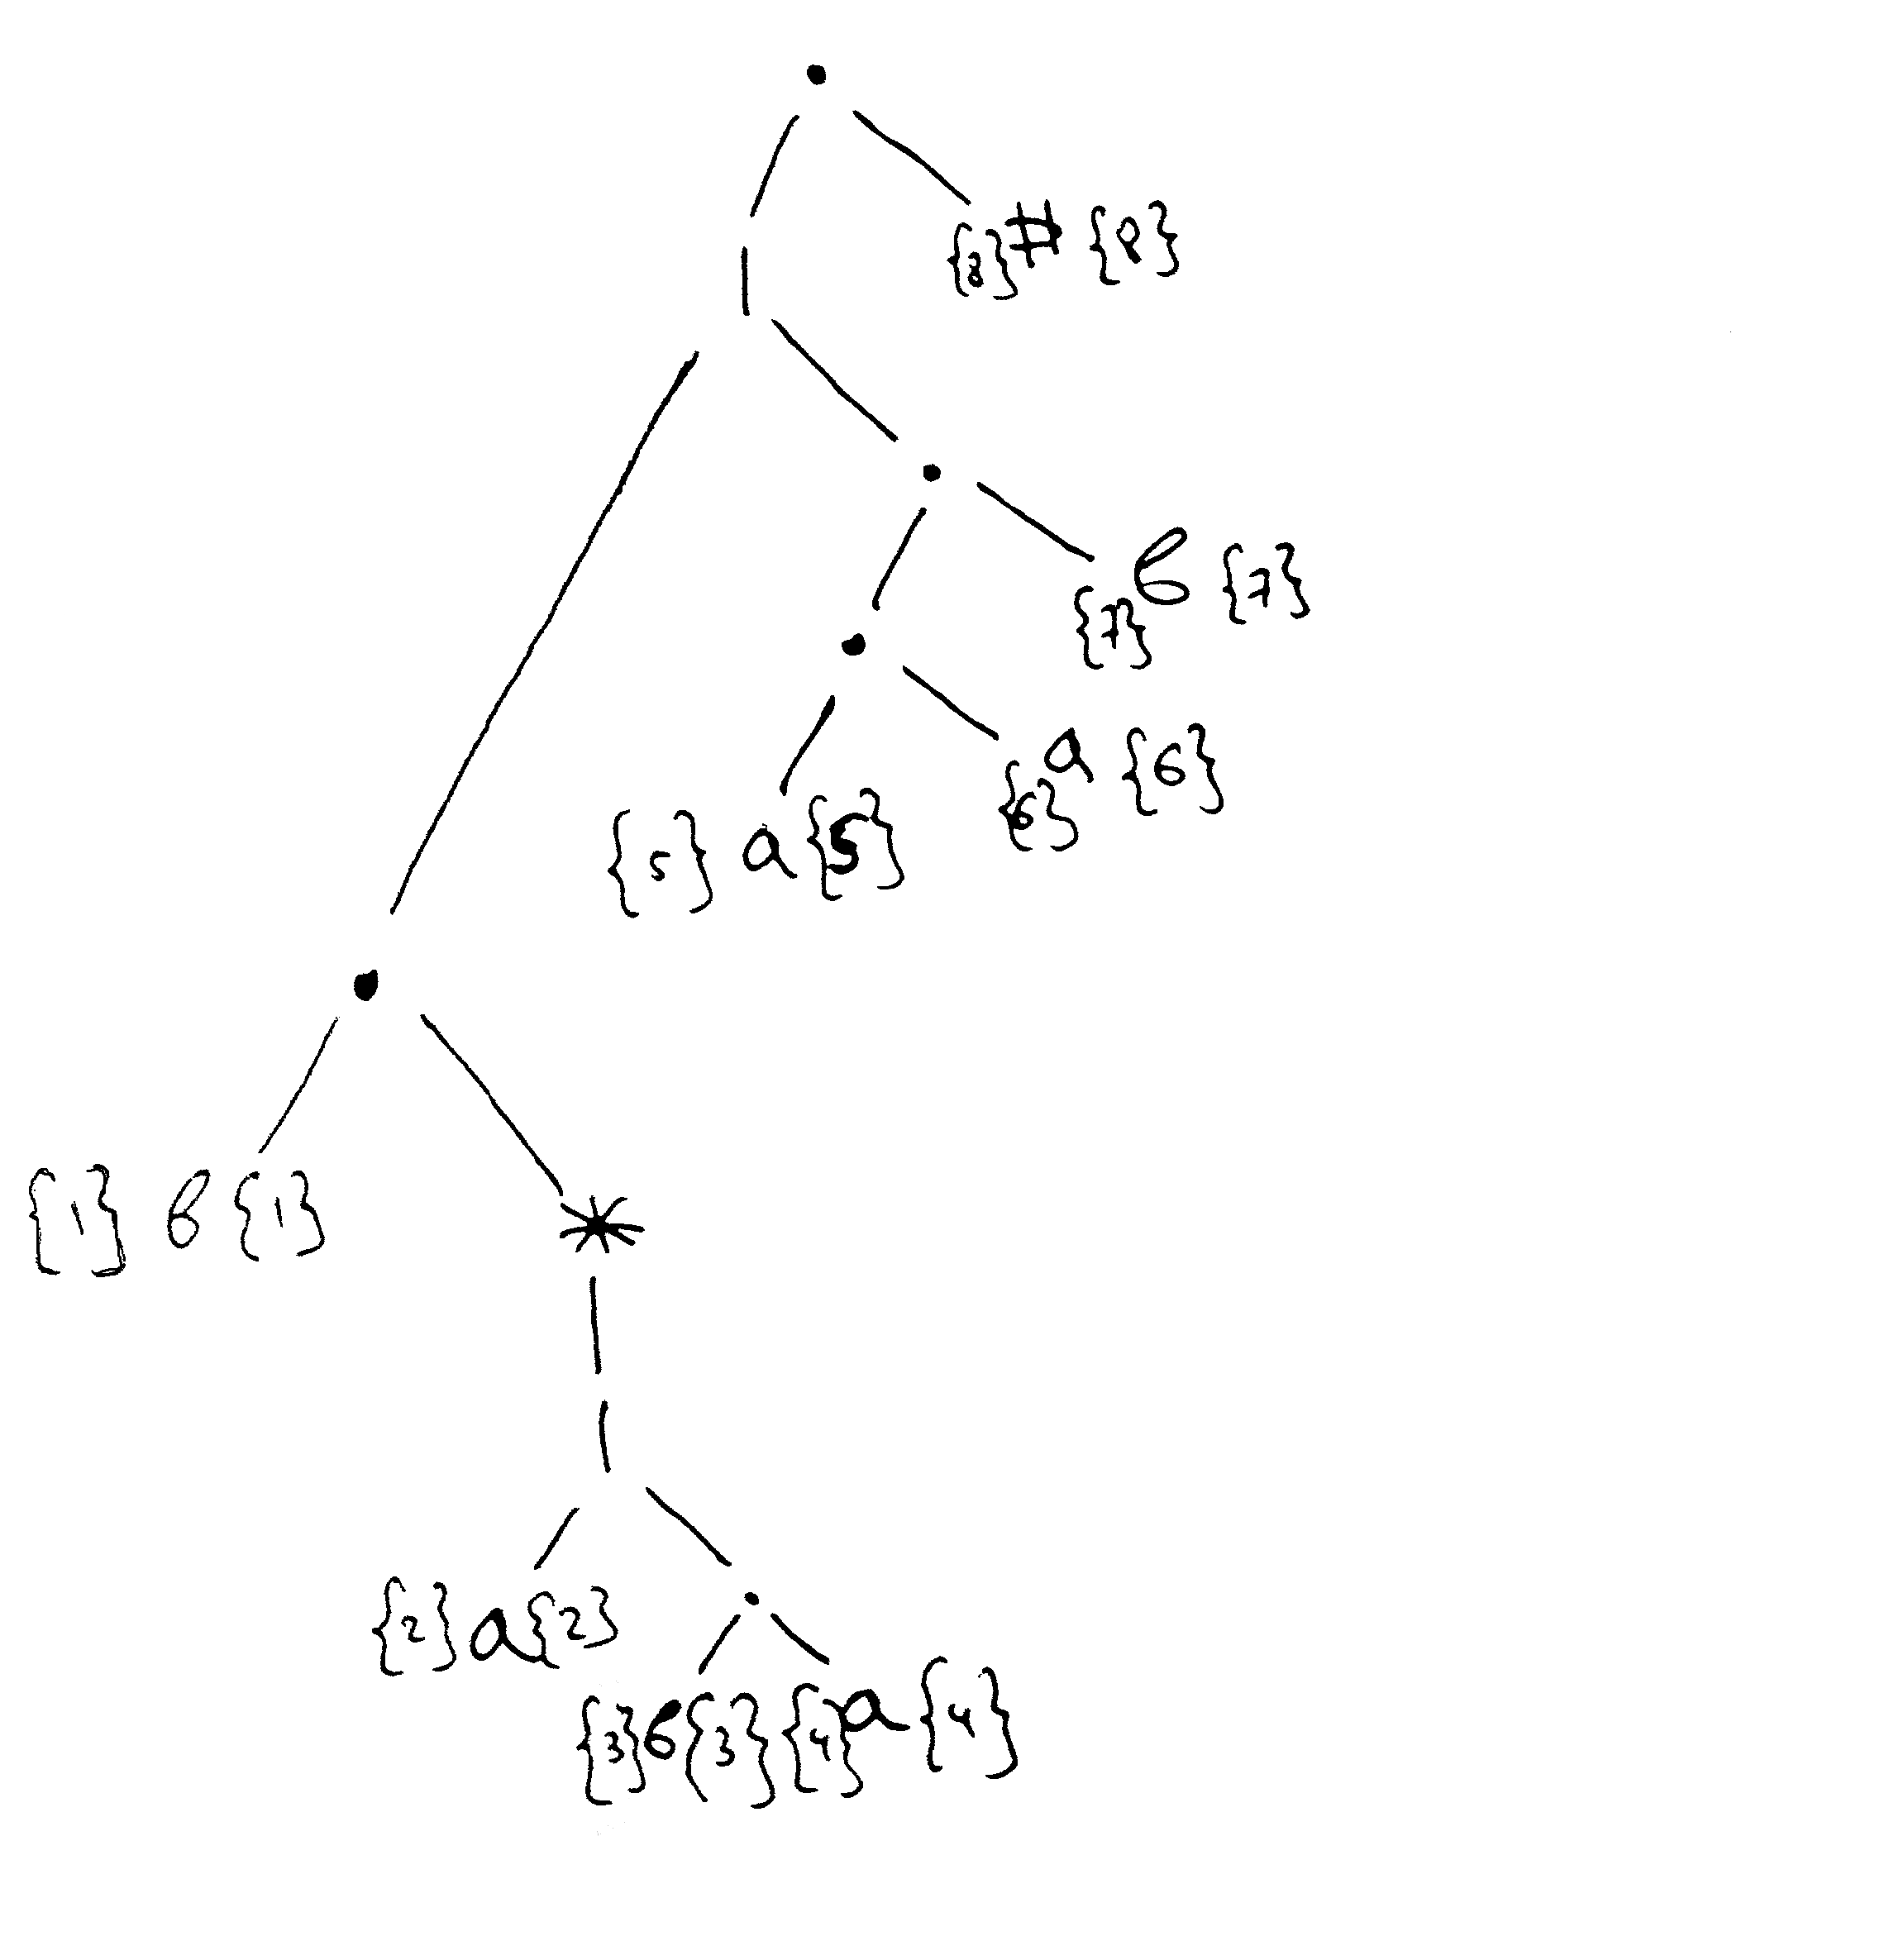
\includegraphics[scale=0.13]{data/pic3_1.png}\\
	4. Теперь пошла жара: надо определить кучу разных множеств для поддеревьев:\\\\
	$nullable(s)$ - обнуляемость: может ли поддерево $s$ породить пустую цепочку\\
	Тут несколько вариантов:\\
	\hspace*{30pt}$s$ - лист дерева: $nullable(s)=false$\\
	\hspace*{30pt}$s=p*$, где $p$ - некоторое поддерево: $nullable(s)=true$\\
	\hspace*{30pt}$s=p\ |\ q$:\ $nullable(s)=nullable(p)\ or\ nullable(q)$\\
	\hspace*{30pt}$s=p \bullet q$:\ $nullable(s)=nullable(p)\ and\ nullable(q)$\\
	$firstpos(s)$ - первый символ: множество символов, которые могут идти первыми
	в цепочке, порожденной поддеревом $s$\\
	\hspace*{30pt}$s$ - лист дерева: $firstpos(s)=\{s\}$\\
	\hspace*{30pt}$s=p*$: $firstpos(s)=firstpos(p)$\\
	\hspace*{30pt}$s=p\ |\ q$: $firstpos(s)=firstpos(p) \cup firstpos(q)$\\
	\hspace*{30pt}$s=p \bullet q$: если $nullable(p)$, то $firstpos(s)=firstpos(p) \cup firstpos(q)$,
	\hspace*{30pt}иначе $firstpos(s)=firstpos(p)$ \\
	$lastpos(s)$ - последний символ: множество символов, на которые может заканчиваться
	цепочка, порожденная поддеревом $s$\\
	\hspace*{30pt}$s$ - лист дерева: $lastpos(s)=\{s\}$\\
	\hspace*{30pt}$s=p*$: $lastpos(s)=lastpos(p)$\\
	\hspace*{30pt}$s=p\ |\ q$: $lastpos(s)=lastpos(p) \cup lastpos(q)$\\
	\hspace*{30pt}$s=pq$: если $nullable(q)$, то $lastpos(s)=lastpos(p) \cup lastpos(q)$,
	\hspace*{30pt}иначе $lastpos(s)=lastpos(q)$ \\\\
	На самом деле все это страшно скучная херня и по большей части решается с помощью метода
	пристального взгляда и более-менее здравого смысла.\\
	Теперь можно пояснить и за странные пометки в предыдущем рисунке: слева стояли $firstpos(s)$,
	а справа - $lastpos(s)$\\
	Cейчас прошлый рисунок будет дополнен аналогичными множествами, но уже не только для листьев.\\
	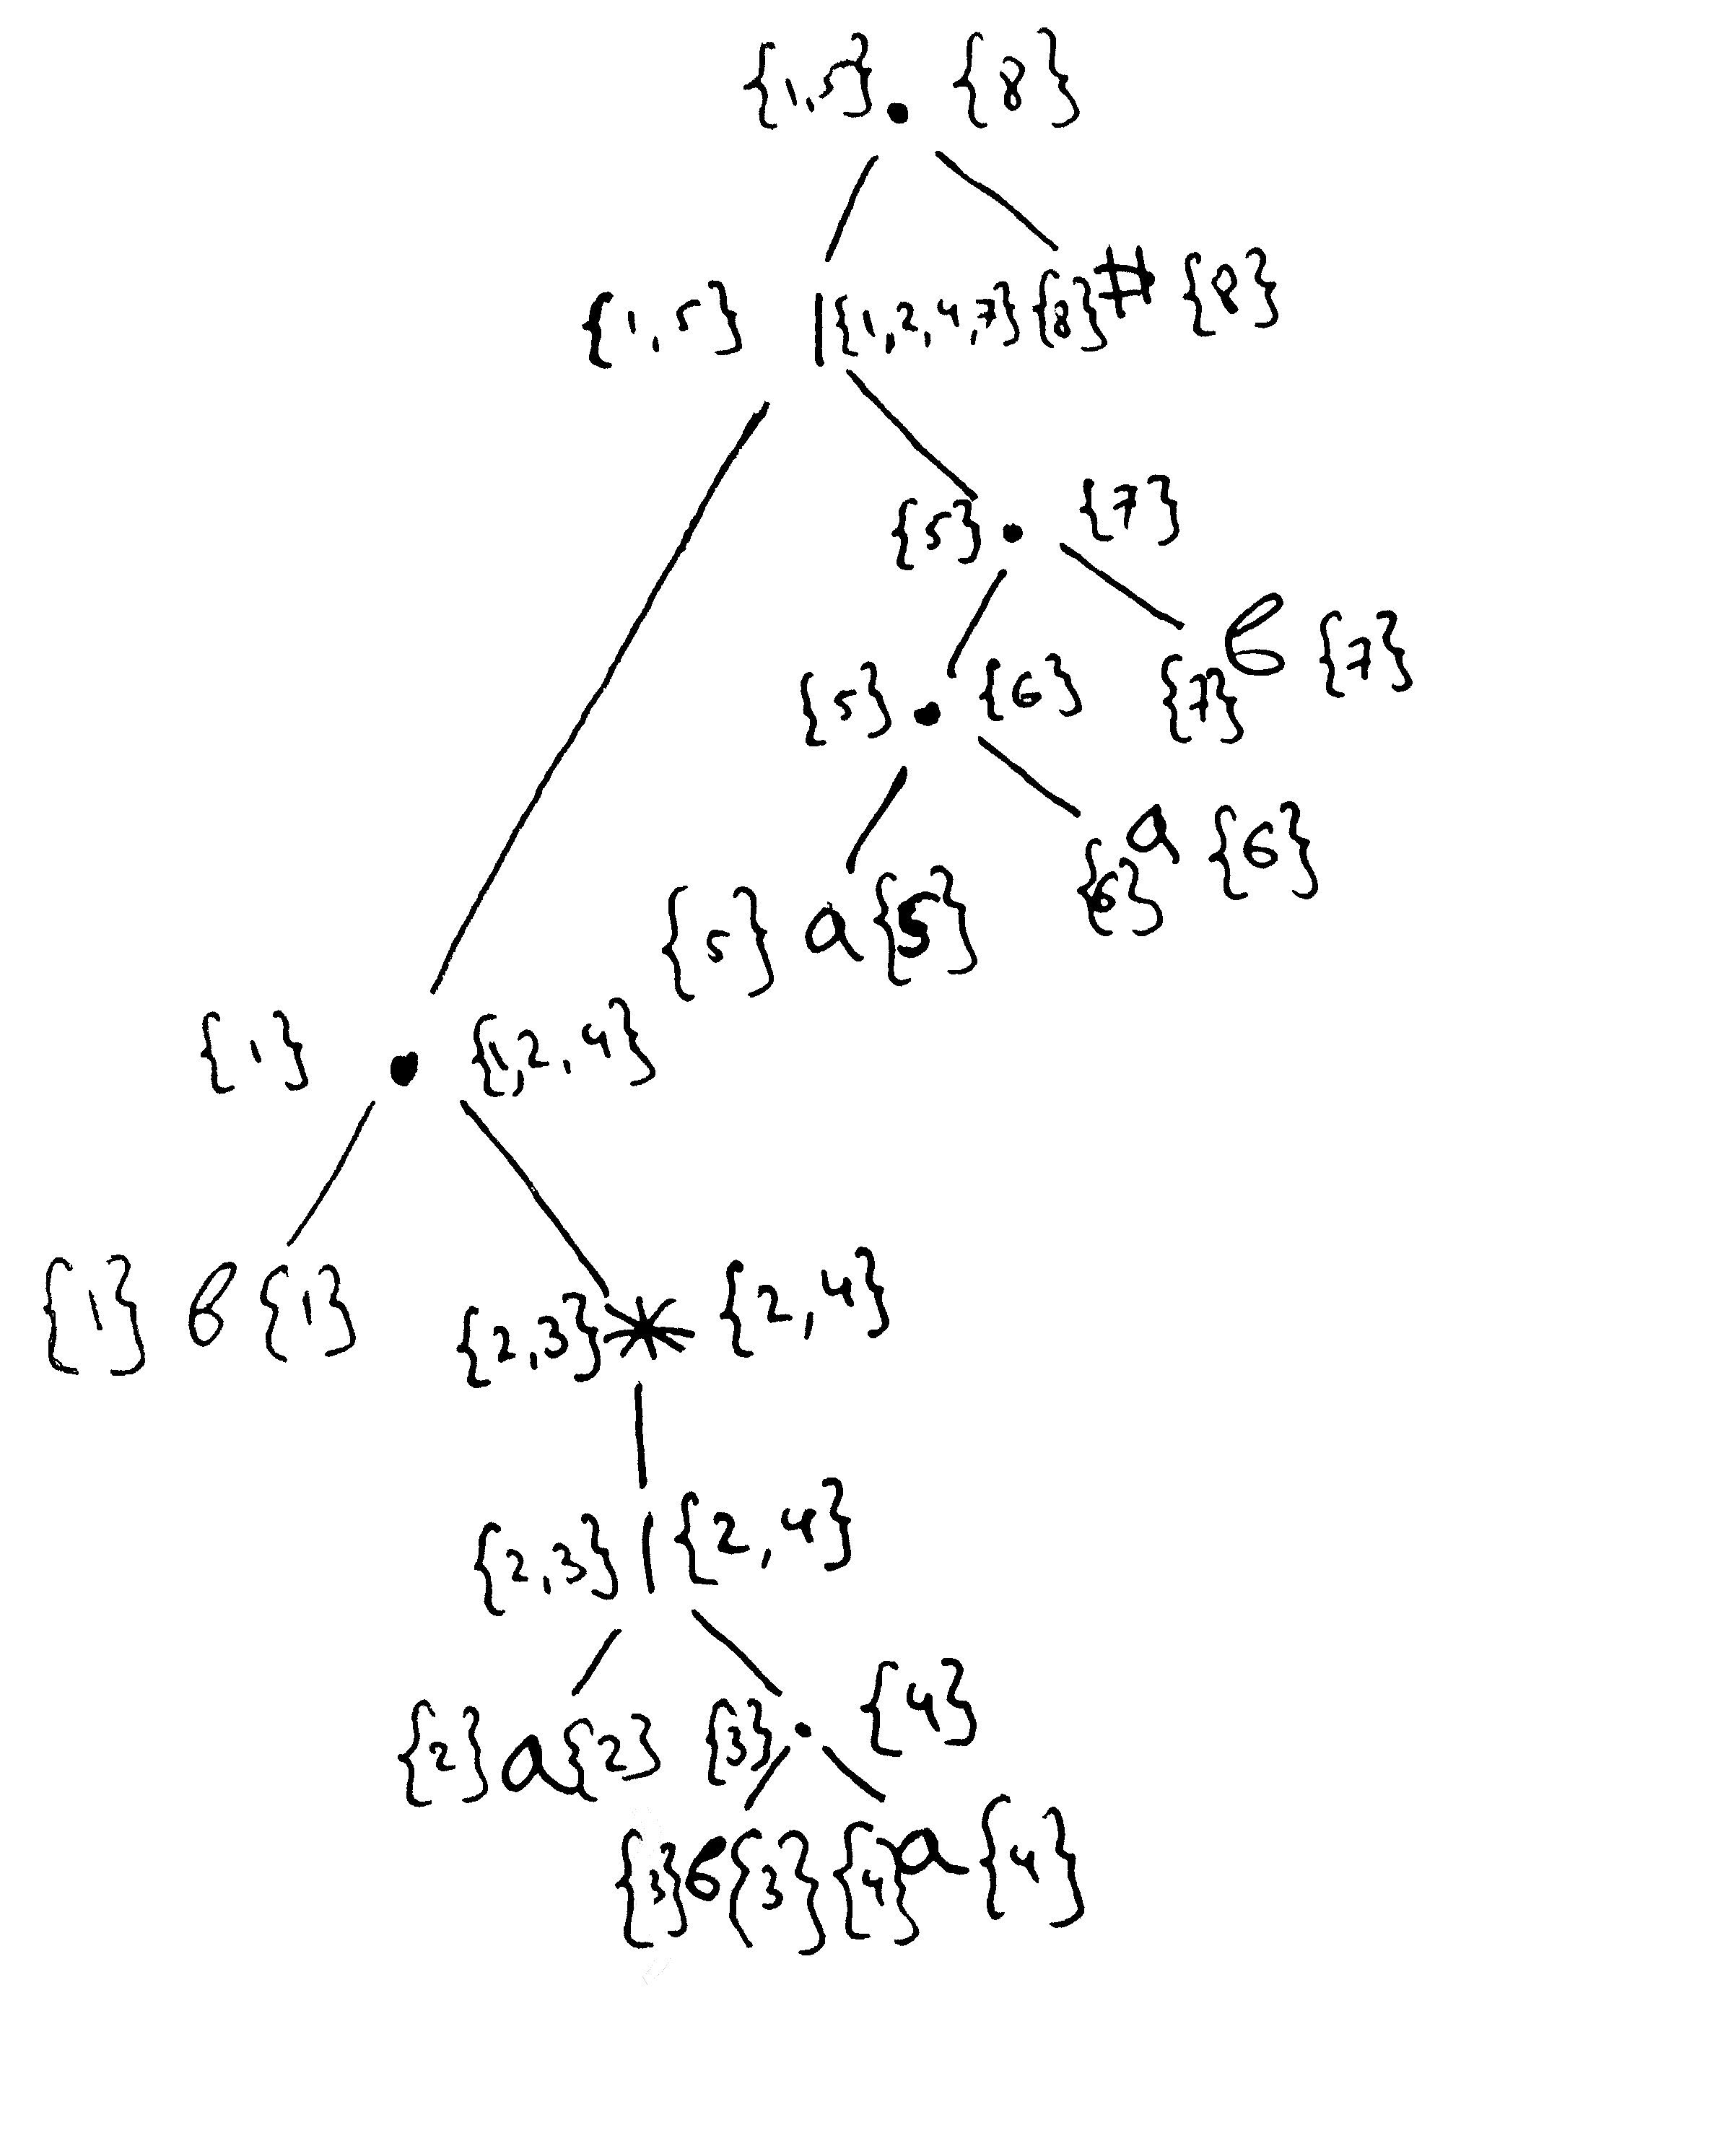
\includegraphics[scale=0.14]{data/pic3_2.png}\\
	5. Жара продолжается: теперь надо вычислить $followpos(s)$ - множество символов, которые могут
	идти прямо после цепочки, порожденной поддеревом $s$.\\
	Здесь строгие алгоритмы выглядят еще скучнее, чем для прошлых множеств, но метод пристального
	взгляда по-прежнему здесь справляется довольно неплохо (хотя иногда и допускает ошибки: мой
	вот пристальный взгляд в свое время накосячил, а теперь я пишу эту методичку).\\
	Но в любом случае, вот алгоритм:\\
	\hspace*{30pt}Для $p \bullet q$: для каждого $i \in lastpos(p)$ добавить $firstpos(q)$
	в $followpos(i)$\\
	\hspace*{30pt}Для  $p*$: для каждой позиции $i \in lastpos(p)$ добавить $firstpos(p)$\\
	\hspace*{30pt}в $followpos(i)$\\
	Вот над вторым правилом очень советую отдельно повтыкать, поразмышлять и полностью осознать,
	как оно получается из метода пристального взгляда: тогда вы, наверное, не накосячите так,
	как однажды это сделал я.\\
	Для нашего дерева получается такая таблица:\\
		\begin{tabular}{ll}
			 $symbol$ & $followpos(symbol)$ \\
			 1 & $\{2, 3, 8\}$ \\
			 2 & $\{2, 3, 8\}$ \\
			 3 & $\{4\}$ \\
			 4 & $\{2, 3, 8\}$ \\
			 5 & $\{6\}$ \\
			 6 & $\{7\}$\\
			 7 & $\{8\}$\\
			 8 & $\{\}$\\
		\end{tabular}\\
	6. Строим таблицу переходов. Состояния здесь описываются множествами, как и в прошлой главе.
	За начальное состояние $A$ берется множество $firstpos($корень дерева$)$.\\
	Дальше правила переходов описываются следующим образом:\\
	$D(Q, s) = \bigcup\limits_{i=Q \cap s}followpos(i)$\\
	Сложная формула, за которой хрен пойми какая логика стоит, поэтому рассмотрим на живом
	примере:\\
	В данном случае наше стартовое состояние $A=\{1, 5\}$.\\
	Символ $a=\{2, 4, 5, 6\}$(множество	цифр, которые в пронумерованном РВ 
	стоят под символом $a$)\\
	Пересекая множества $a$ и$A$ получим $\{5\}$. $followpos(5)$ смотрим по таблице -
	$\{6\}$. Такого множества в качестве состояния у нас еще не было, поэтому назовем его
	$B=\{6\}$. Таким образом получается, что $D(A, a) = B$.\\
	Абсолютно аналогично поступаем со всеми символами алфавита и всеми неописанными множествами.
	Со временем новые состояния перестанут поступать, а мы получим законченную таблицу.\\
	Конечным состоянием объявляется то, которое в своем множестве содержит номер символа конца.\\
	\newpage
	Для нашего $b(a|ba)*|aab$ получается следующая таблица:\\
		\begin{tabular}{lcc}
			 & $a\{2, 4, 5, 6\}$ & $b\{1, 3, 7\}$ \\
			 $A\{1, 5\}$ & $B$ & $C$ \\
			 $B\{6\}$ & $D$ & x \\
			 $*C\{2, 3, 8\}$ & $C$ & $E$ \\
			 $D\{7\}$ & x & $F$ \\
			 $E\{4\}$ & $C$ & x \\
			 $*F\{8\}$ & x & x \\
		\end{tabular}\\
	Осталось всего ничего: построить сам ДКА по таблице\\
	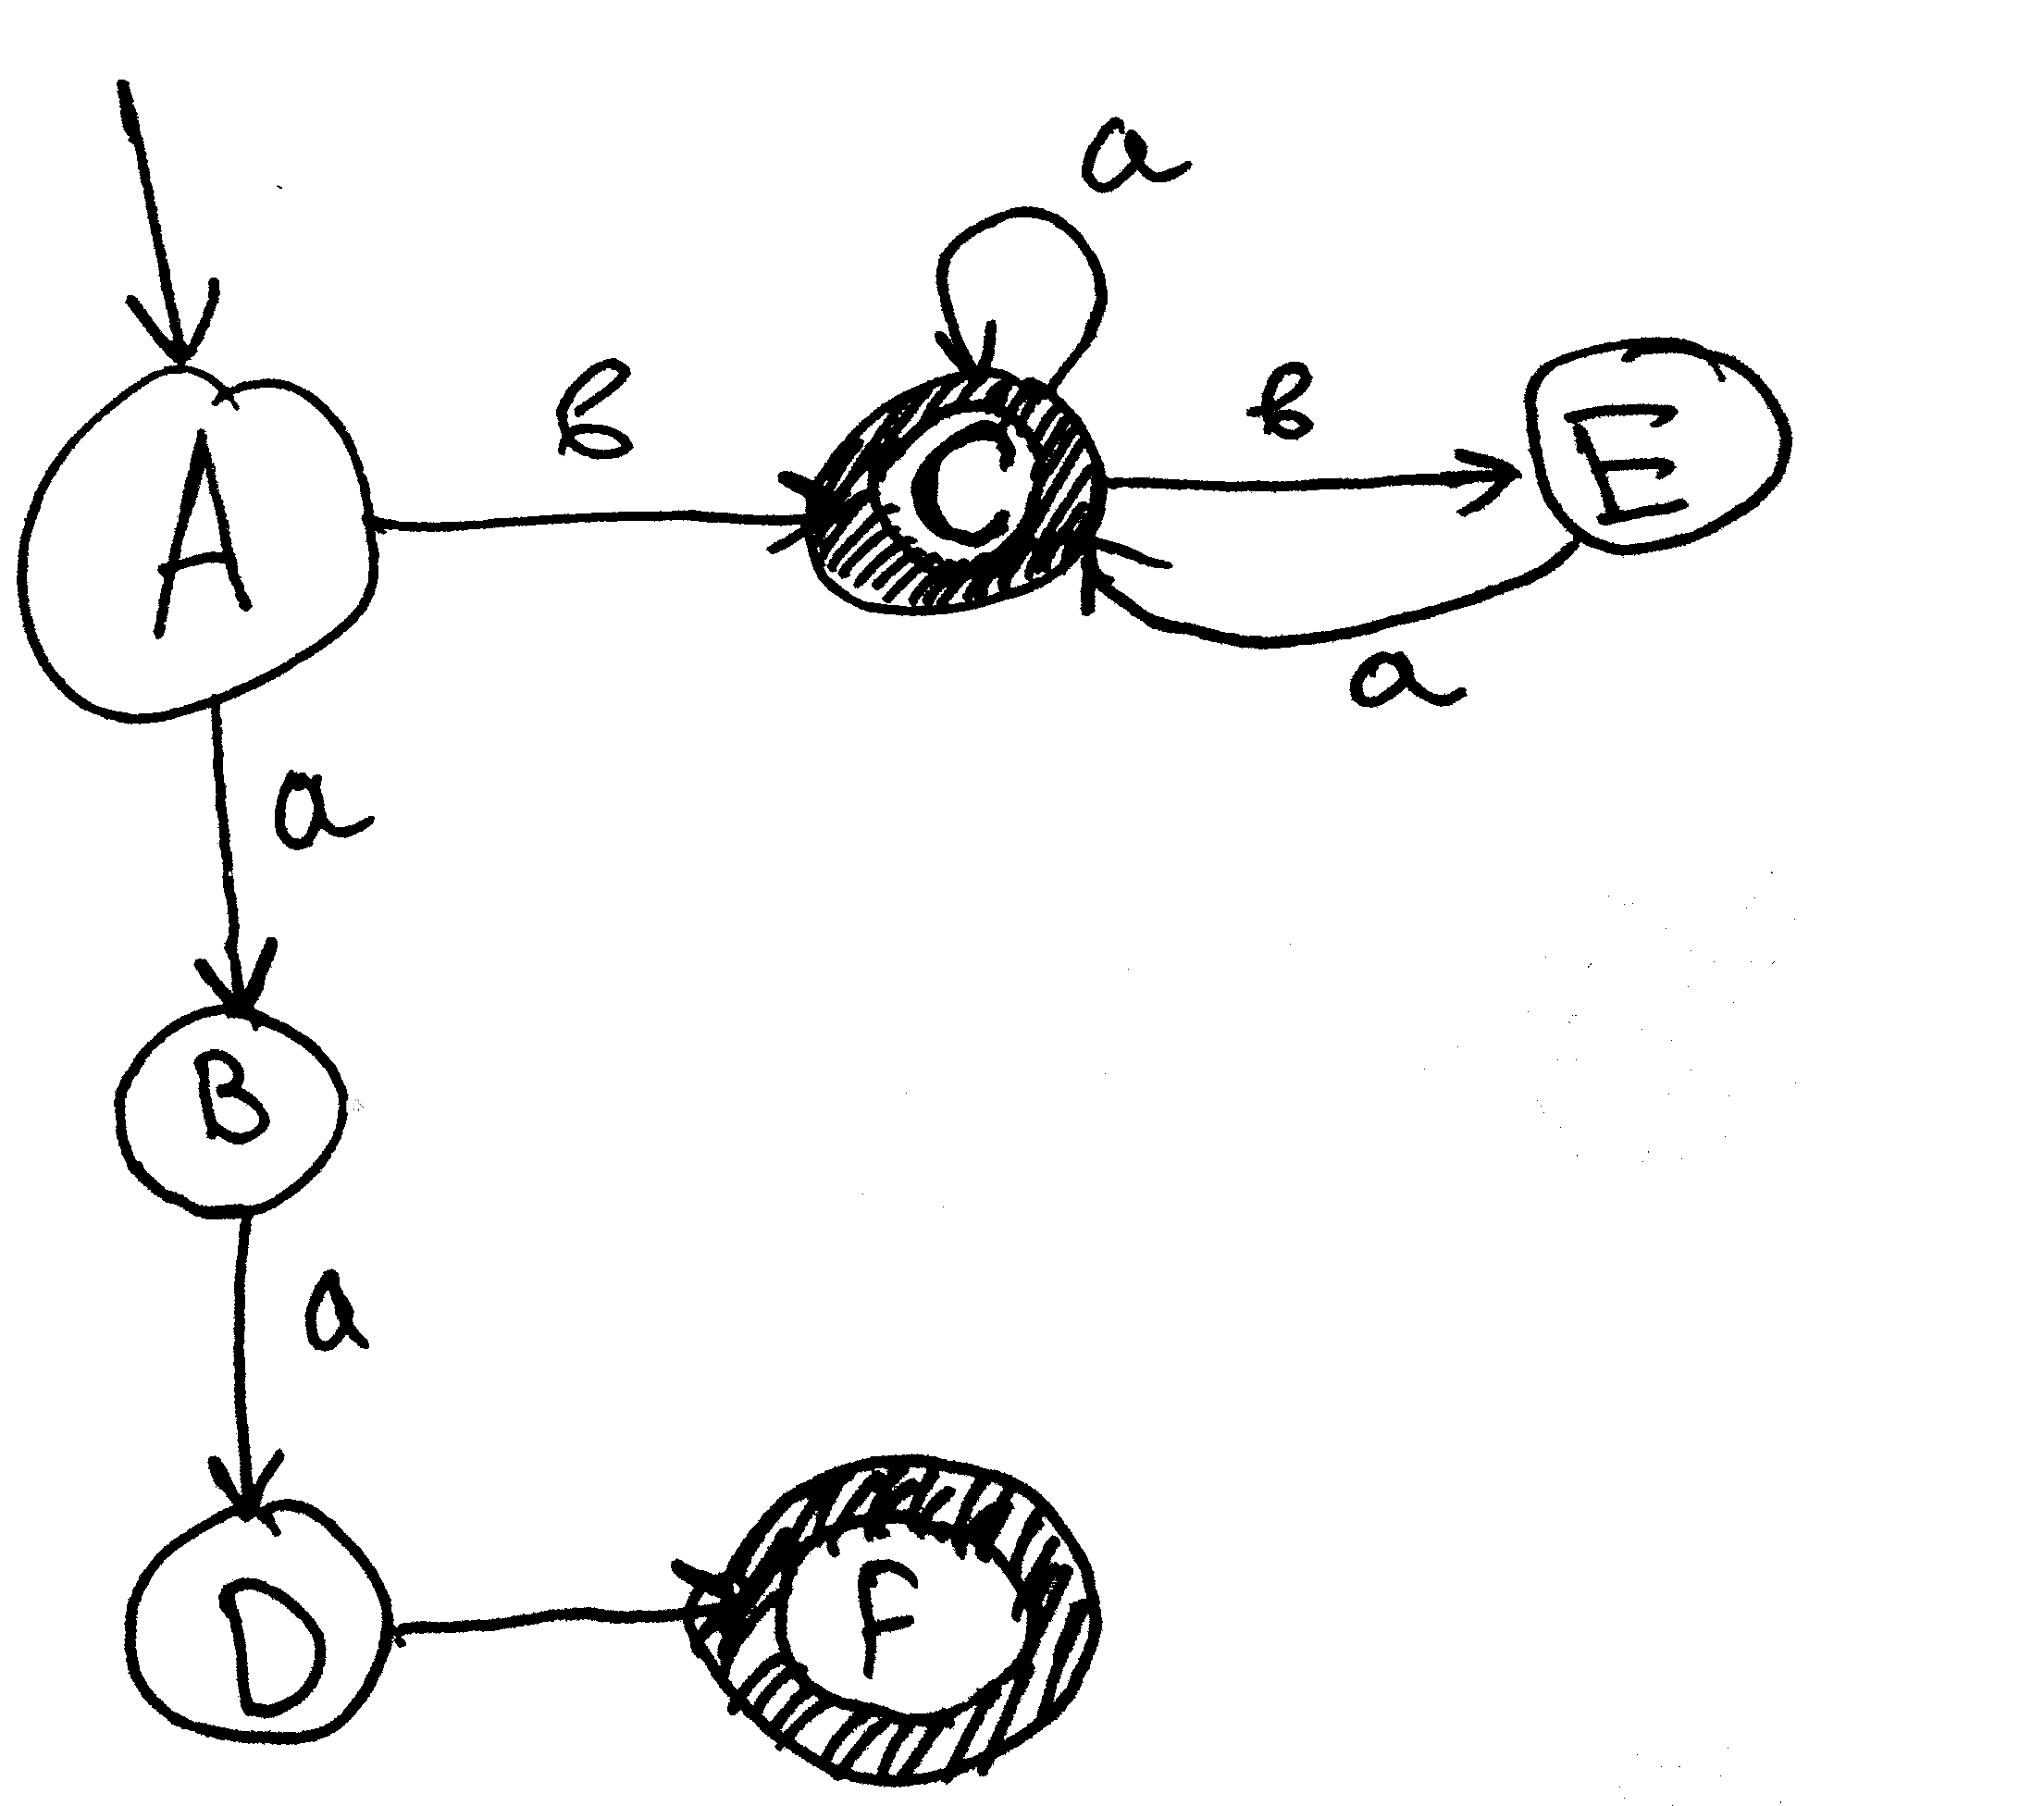
\includegraphics[scale=0.11]{data/pic3_3.png}\\
	\section{Почему это работает}
	По сути каждое состояние описано множеством тех номеров букв, которые могут нас из
	этого состояния вывести. Действительно, если внимательно посмотреть на наше РВ,\\
	$(b(a|ba)*|aab)\#$\\
	\hspace*{5pt}$1\ 2\ 34\ \ \ \ \ 567\ 8$\\
	можно заметить, что выйти из начального состояния мы можем только по буквам $b1$ и $a5$.
	При этом те же буквы, но с другими номерами нам не подойдут. $followspos$-ы здесь тоже
	появляются вполне по делу: через них очень удобно описываются те номера букв, которые выводят
	нас из состояния, в котором мы оказались. Ведь если мы уже прошли вперед по символу $b1$, то
	дальше в цепочке, удовлетворящей РВ, мы по определению сможем встретить только символ из
	$followpos(b1)$.\\
	Из всех этих номеров можно построить очень простой, но здоровый автомат разбора, где алфавит
	нетерминалов будет состоять из чисел, которыми нумеруются буквы в исходном РВ. Просто этот
	большой автомат потом можно будет сократить, заменив номера, на буквы, которые им
	соответствуют.
	\newpage
	\chapter{Минимизация ДКА}
	Внимательный читатель мог задаться вопросом: как же так получилось, что мы взяли
	одно РВ, и получилось 2 разных ДКА? И почему это второй ДКА получился таким аккуратным?\\
	А все потому, что ДКА из НКА мы не минимизировали.
	\section{Алгоритм}
	1. Первым делом автомат надо дополнить, то есть, сделать так, чтобы в нем всегда было куда
	перейти (сделаем так, чтобы не было правил вида $D(Q, s) = \O$)\\
	Если автомат уже полный, то ничего не делаем, в противном случае добавляем новое состояние
	$V$ (ну или как вы его назовете, я называю $V$ от слова $void$, потому что это удобно), а
	после этого ведете в него все отсутствующие дуги (и из $V$ в себя же по всем буквам
	алфавита).\\
	В качестве примера возьмем нашего старого доброго уродца из "НКА по РВ" и дополним его:\\
	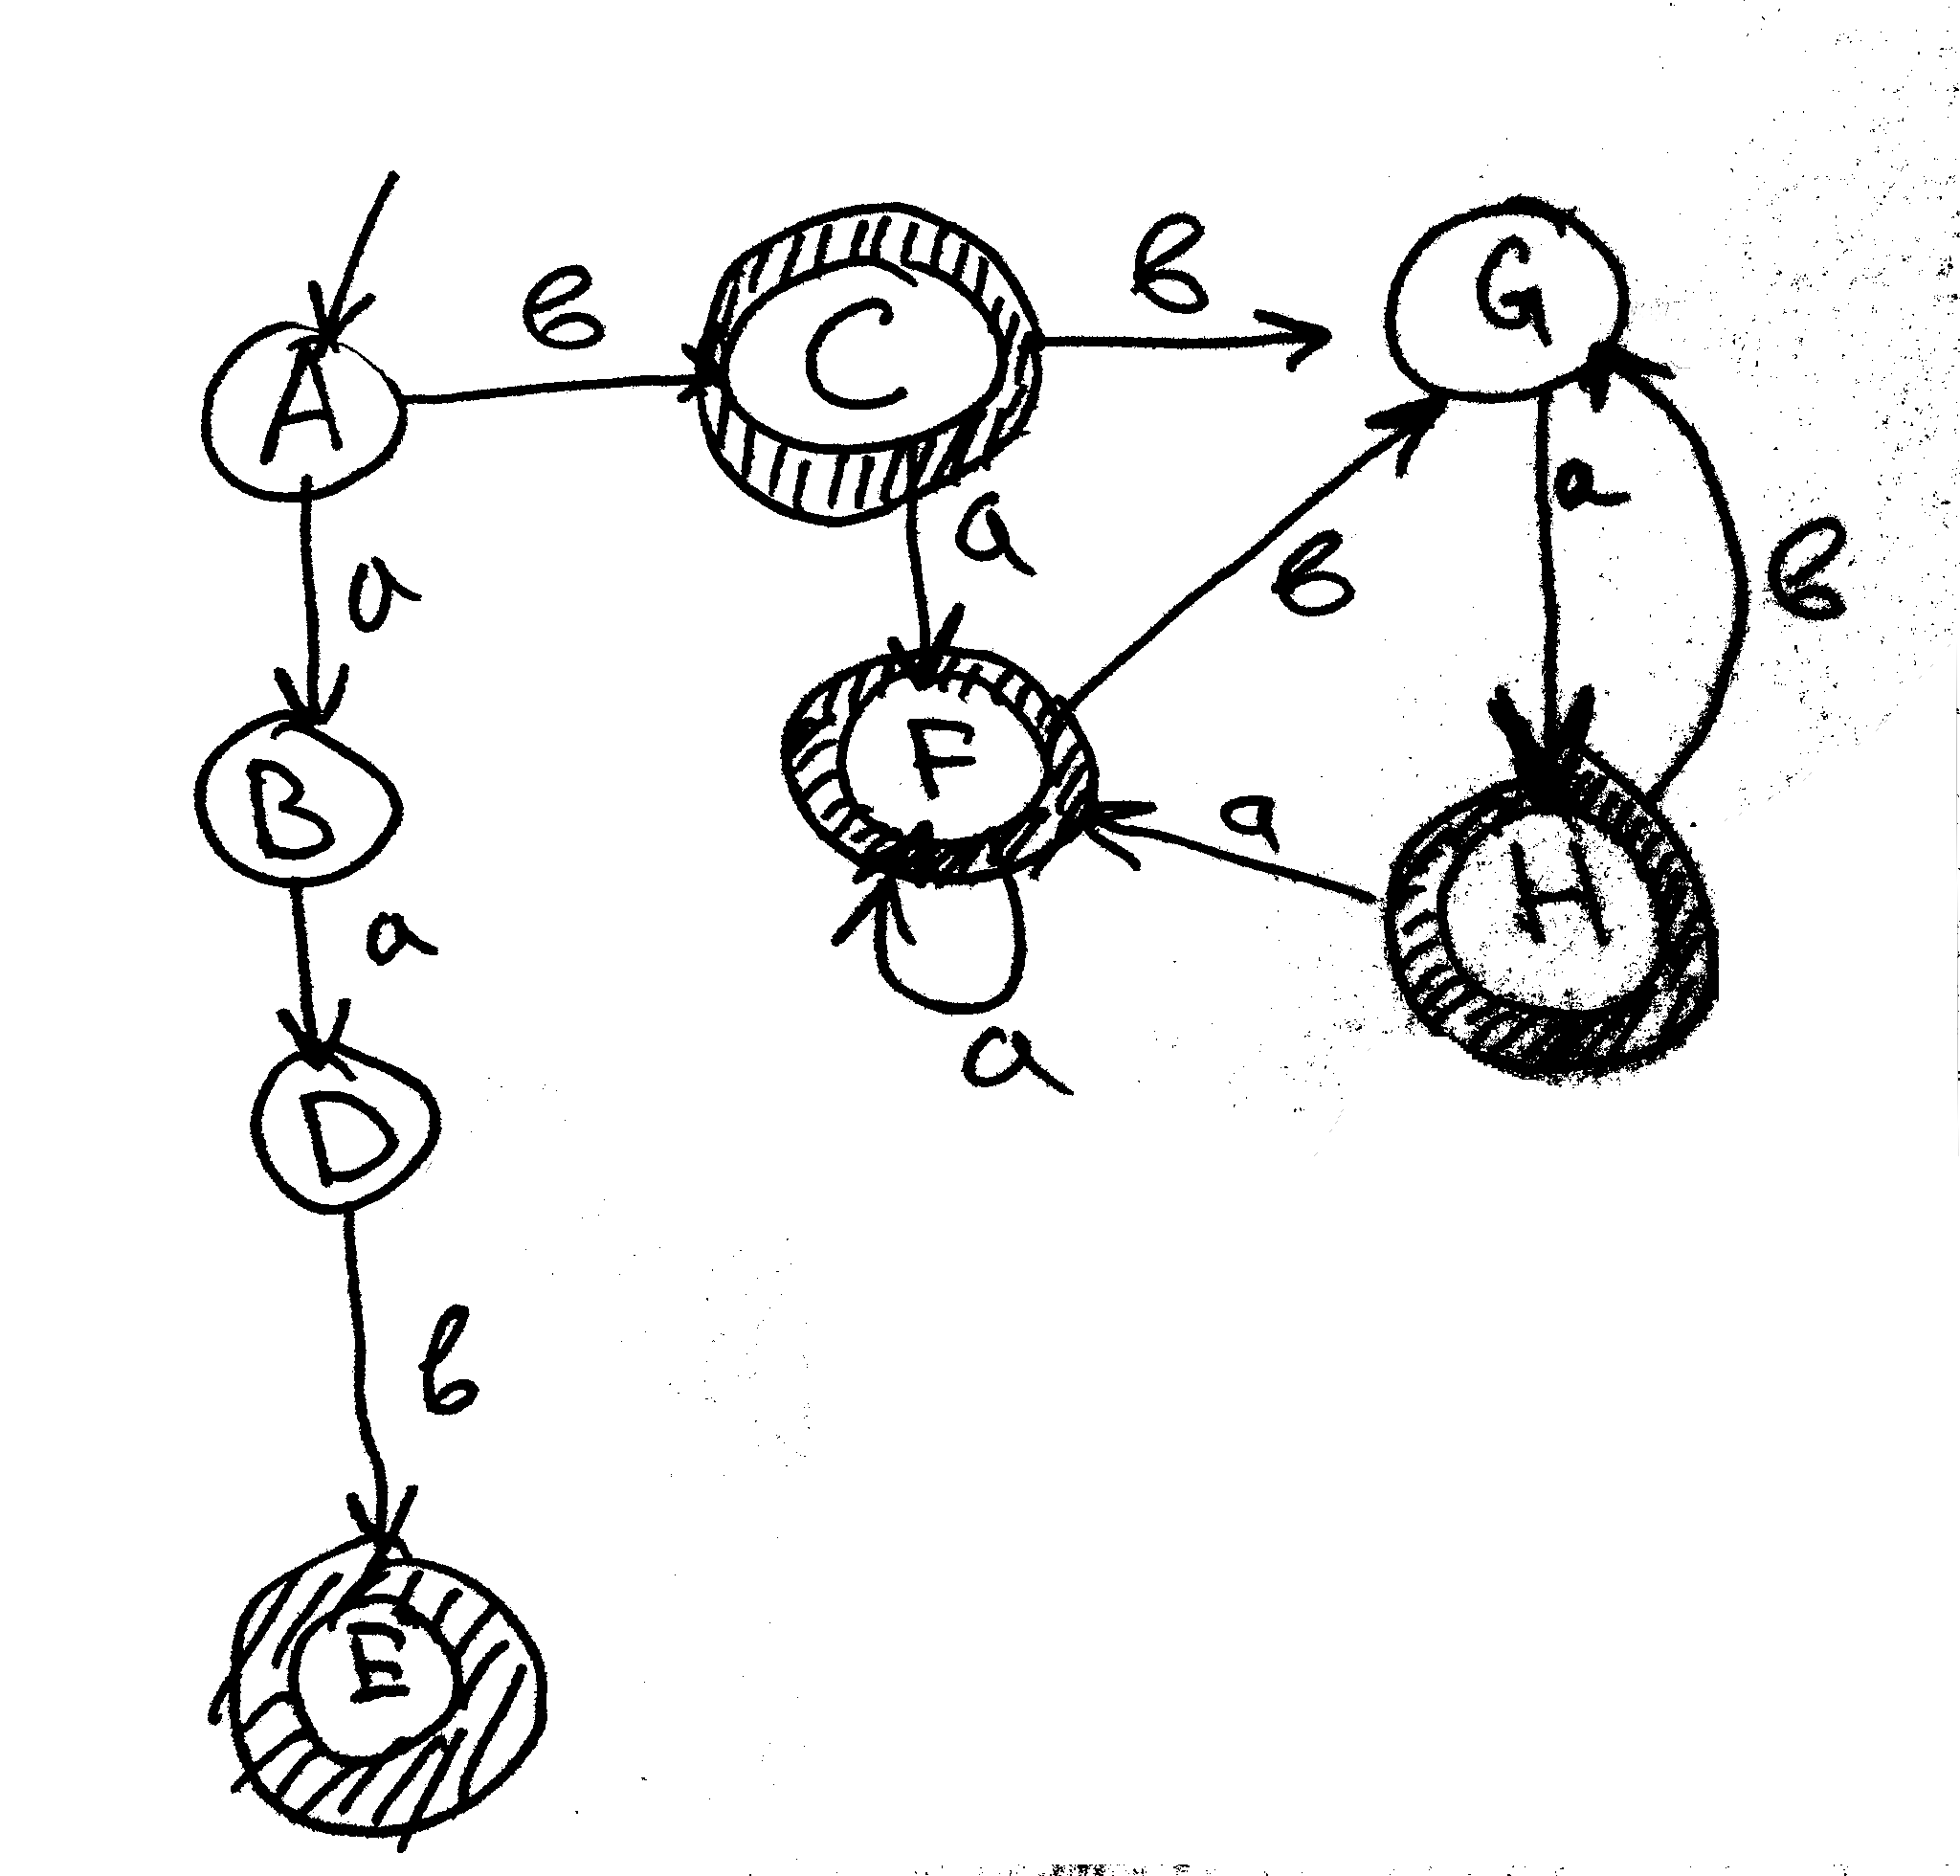
\includegraphics[scale=0.1]{data/pic2_2.png} 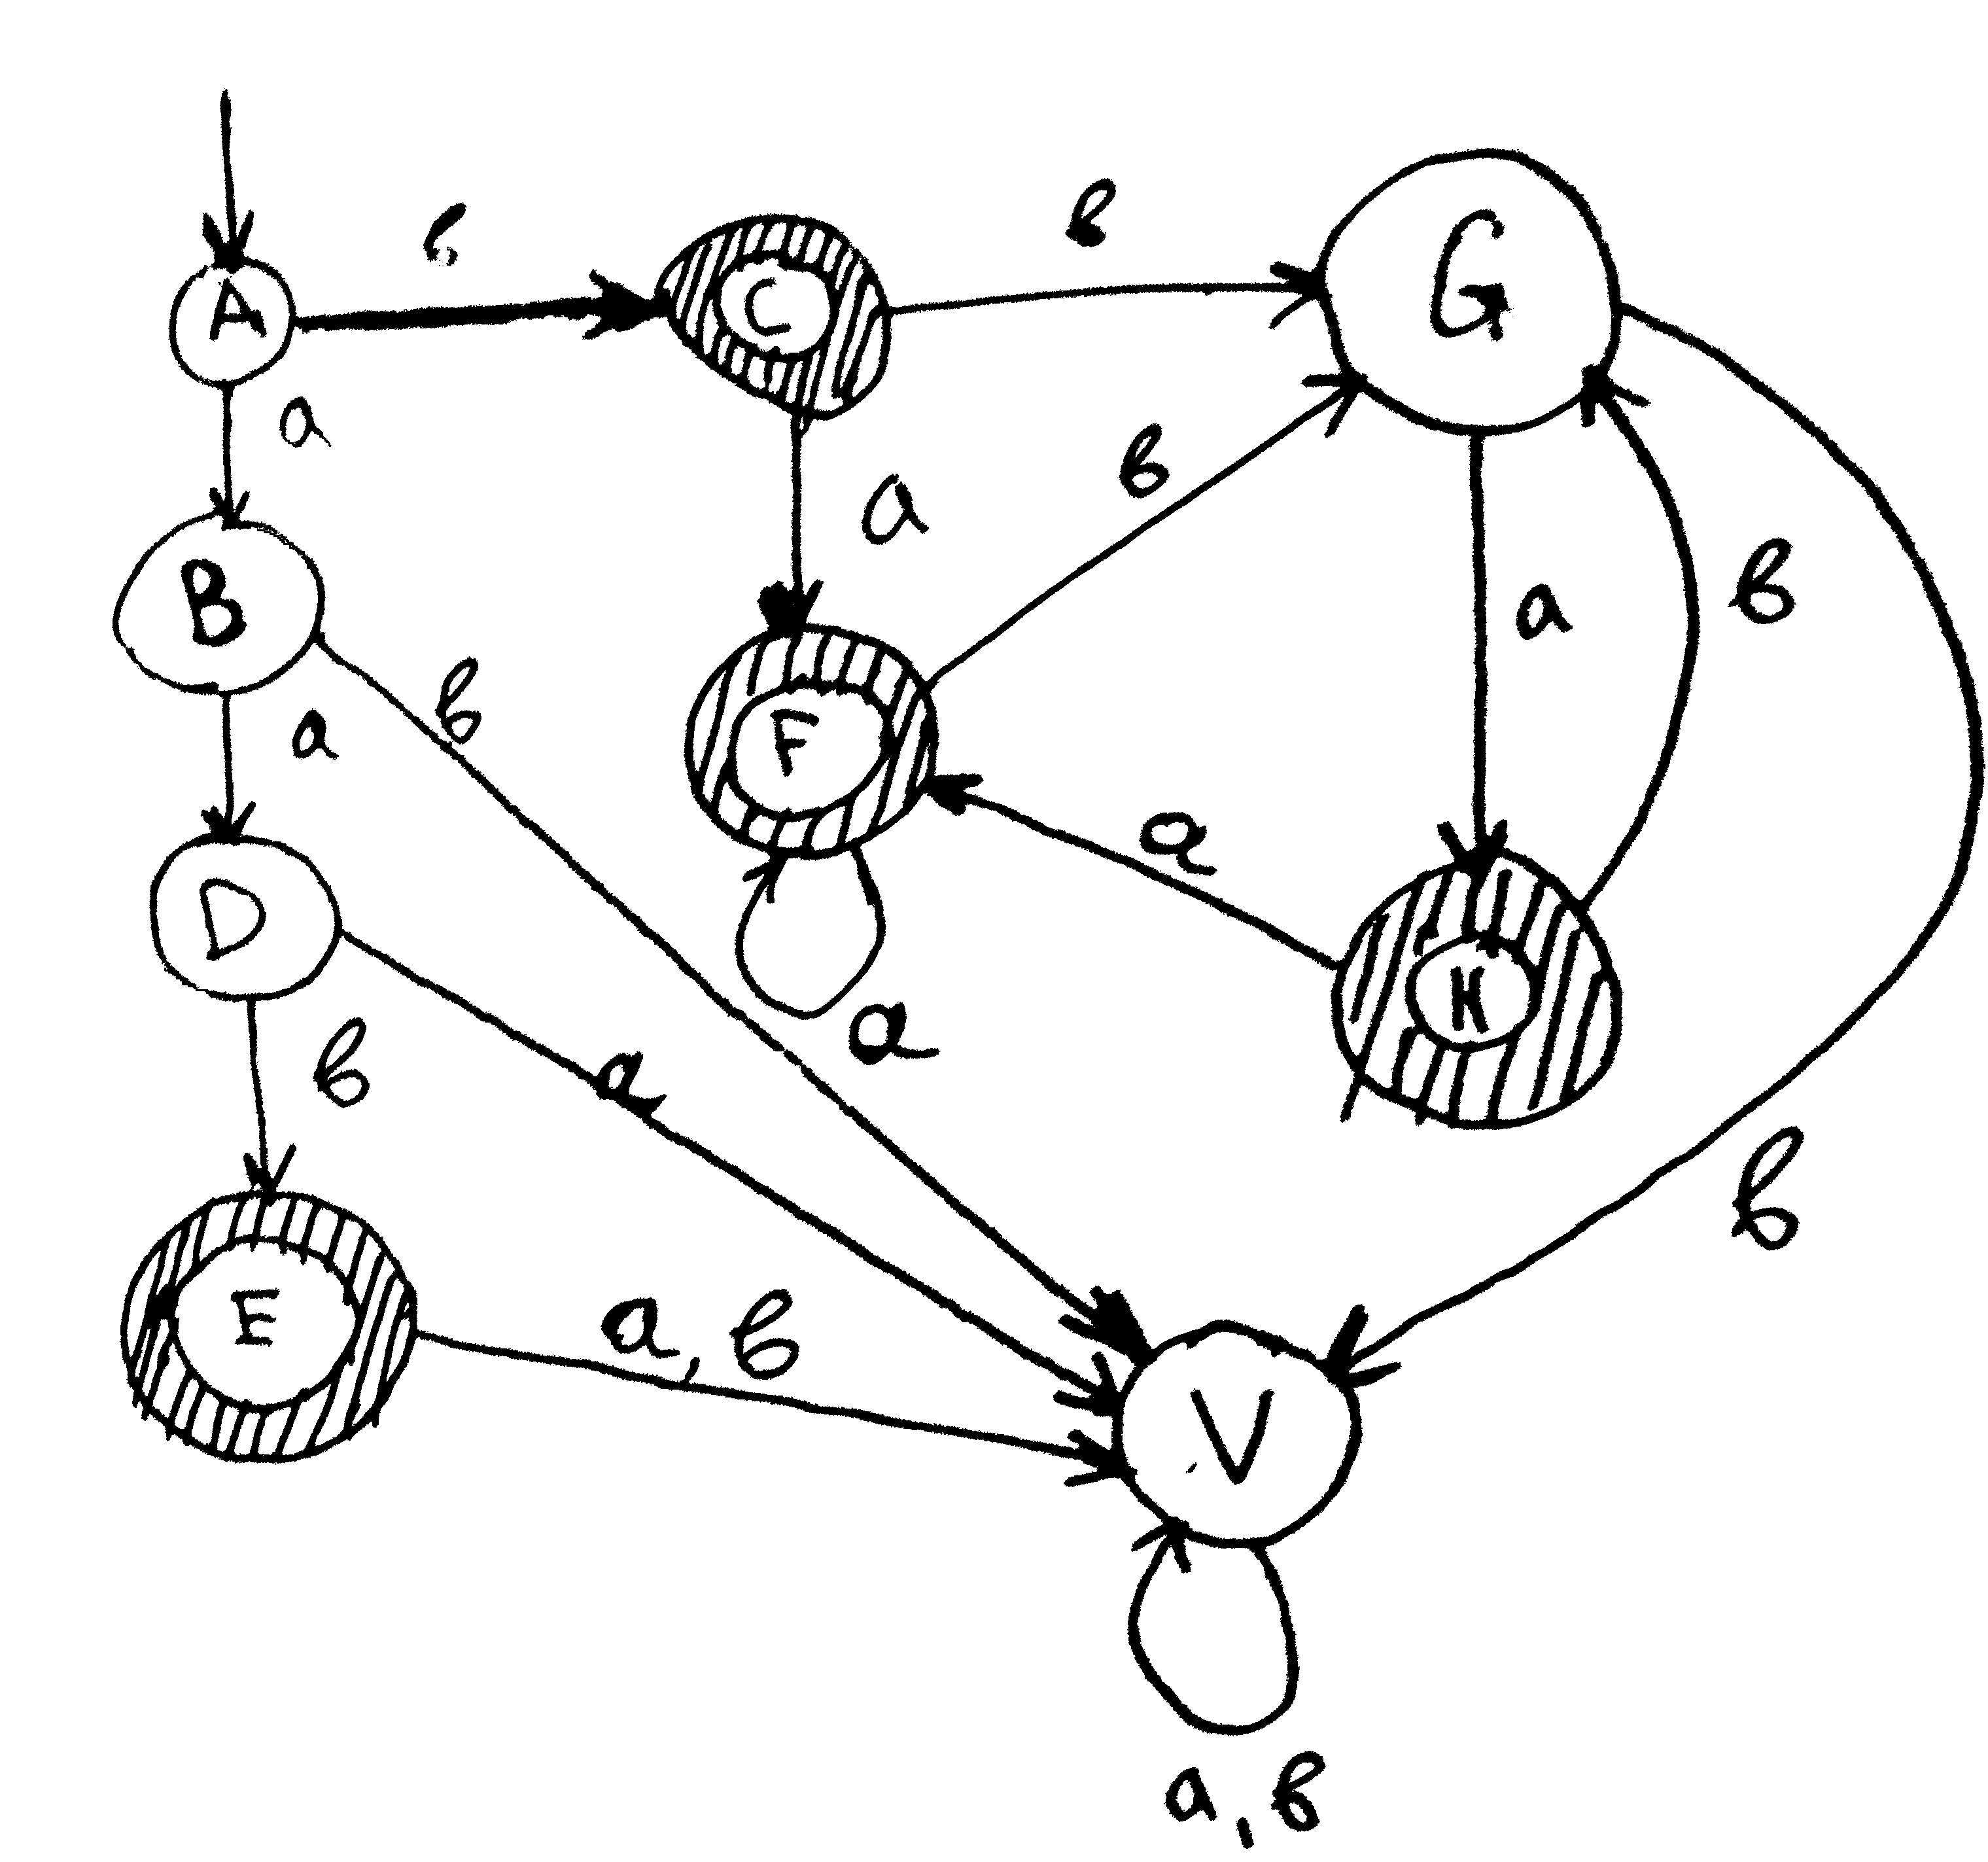
\includegraphics[scale=0.08]{data/pic4_1.png}
	\\\\
	2. Строим разбиение $P_{0}$ множеств состояний следующим образом:\\
	$P_{0}=\{F\},\{Q \setminus F\}$, где $\{F\}$ - все конечные состояния,
	а $\{Q \setminus F\}$ - все остальные. В дальнейшем эти множества я буду называть
	группами.\\
	А дальше строится разбиение $P_1$ следующим образом:\\
	Если $A$ и $B$ принадлежает одной группе и по всем нетерминальным символам
	переходят в одну и ту же группу (не обязательно в свою), то они остаются
	в одной группе. А если есть два состояния из одной группы, и по какому-то нетерминалу
	переходит в другую группу, то он уходит в новую группу.\\
	И вот все эти разбиения надо продолжать до тех пор, пока не окажется, что $P_{n}=P_{n+1}$
	(умные люди называют это стабилизацией).\\\\
	Рассмотрим отдельный пример:\\
	$P_0=\{S\}, \{A, B, C, D\}$, при этом $A, B$ по символу $a$ переходят в $\{S\}$, а по
	$b$ - в свою группу. $C, D$ же по $a, b$ переходят в свою группу. И тут можно сначала
	выделить отдельную группу $\{A\}$, а потом еще одну группу $\{B\}$. На самом деле группа
	определяется тем, что ее элементы ведут себя одинаково, а в данном случае $A$ и $B$ ведут
	себя идентично, поэтому правильнее будет выделить их вместе в отдельную группу и получить
	разбиение $P_1=\{S\},\{A,B\},\{C,D\}$. Если вдруг выяснится, что $A$ и $B$ на самом деле
	ведут себя по-разному, то на следующих итерациях, они будут разведены по разным группам,
	но пока что они должны быть в одной группе. За такими удалениями разных элементов в одну
	группу надо внимательно следить, иначе можно получить ошибочный ответ.\\\\
	А теперь мы построим разбиения на группы для нашего дополненного автомата:\\
	При этом у каждой группы я буду ставить ее порядковый номер, а возле состояний в группе
	буду ставить "вектор переходов в группы". Поясню за сложное словосочетание
	"вектор переходов в группы": $A_{03}$ означает,
	что по $a$ мы переходим из $A$ в группу-0, а по $b$ - в группу-3. Так сразу становится
	понятно, кого надо разнести по разным группам, а кого надо оставить в одной.\\\\
	$P_0=\{C_{01}, E_{11}, F_{01}, H_{01}\}_0,\{A, B, D, G, V\}_1$\\
	$P_1=\{C, F, H\}_0,\{E\}_1,\{A_{20}, B_{22}, D_{21}, G_{02}, V_{22}\}_2$\\
	$P_2=\{C, F, H\}_0,\{E\}_1,\{A\}_2,\{B_{43}, V_{33}\}_3, \{D\}_4, \{G\}_5$\\
	$P_3=\{C_{05}, F_{05}, H_{05}\}_0,\{E_{66}\}_1,\{A_{30}\}_2,\{B_{46}\}_3, \{D_{61}
	\}_4, \{G_{06}\}_5, \{V_{66}\}_6$\\
	$P_4=P_3$: закончили\\\\
	\newpage
	Внимательный читатель может подумать, что я охерел и не всегда выставлял
	"вектор переходов в группы"\ у состояний. Это все банально потому, что мне очень лень.
	Не обязательно на одной итерации разносить по разным группам ВСЕ, что только можно.
	Если в одной группе есть два состояния, которые надо разнести по группам, то рано или поздно
	мы все равно до них доберемся и разнесем. А разнося состояния потихоньку, ниже шанс ошибки
	(наверное).\\
	Осталось всего ничего: построить автомат, взяв в качестве состояний группы, и удалив
	бесполодные и недостижимые состояния (те, из которых нет пути в какое-нибудь итоговое
	состояние и те, в которые нет входящих стрелок), это вполне успешно делается методом
	пристального взгляда. 
	Бесплодным состоянием как минимум является состояния, содержащее наше новое состояние $V$.\\
	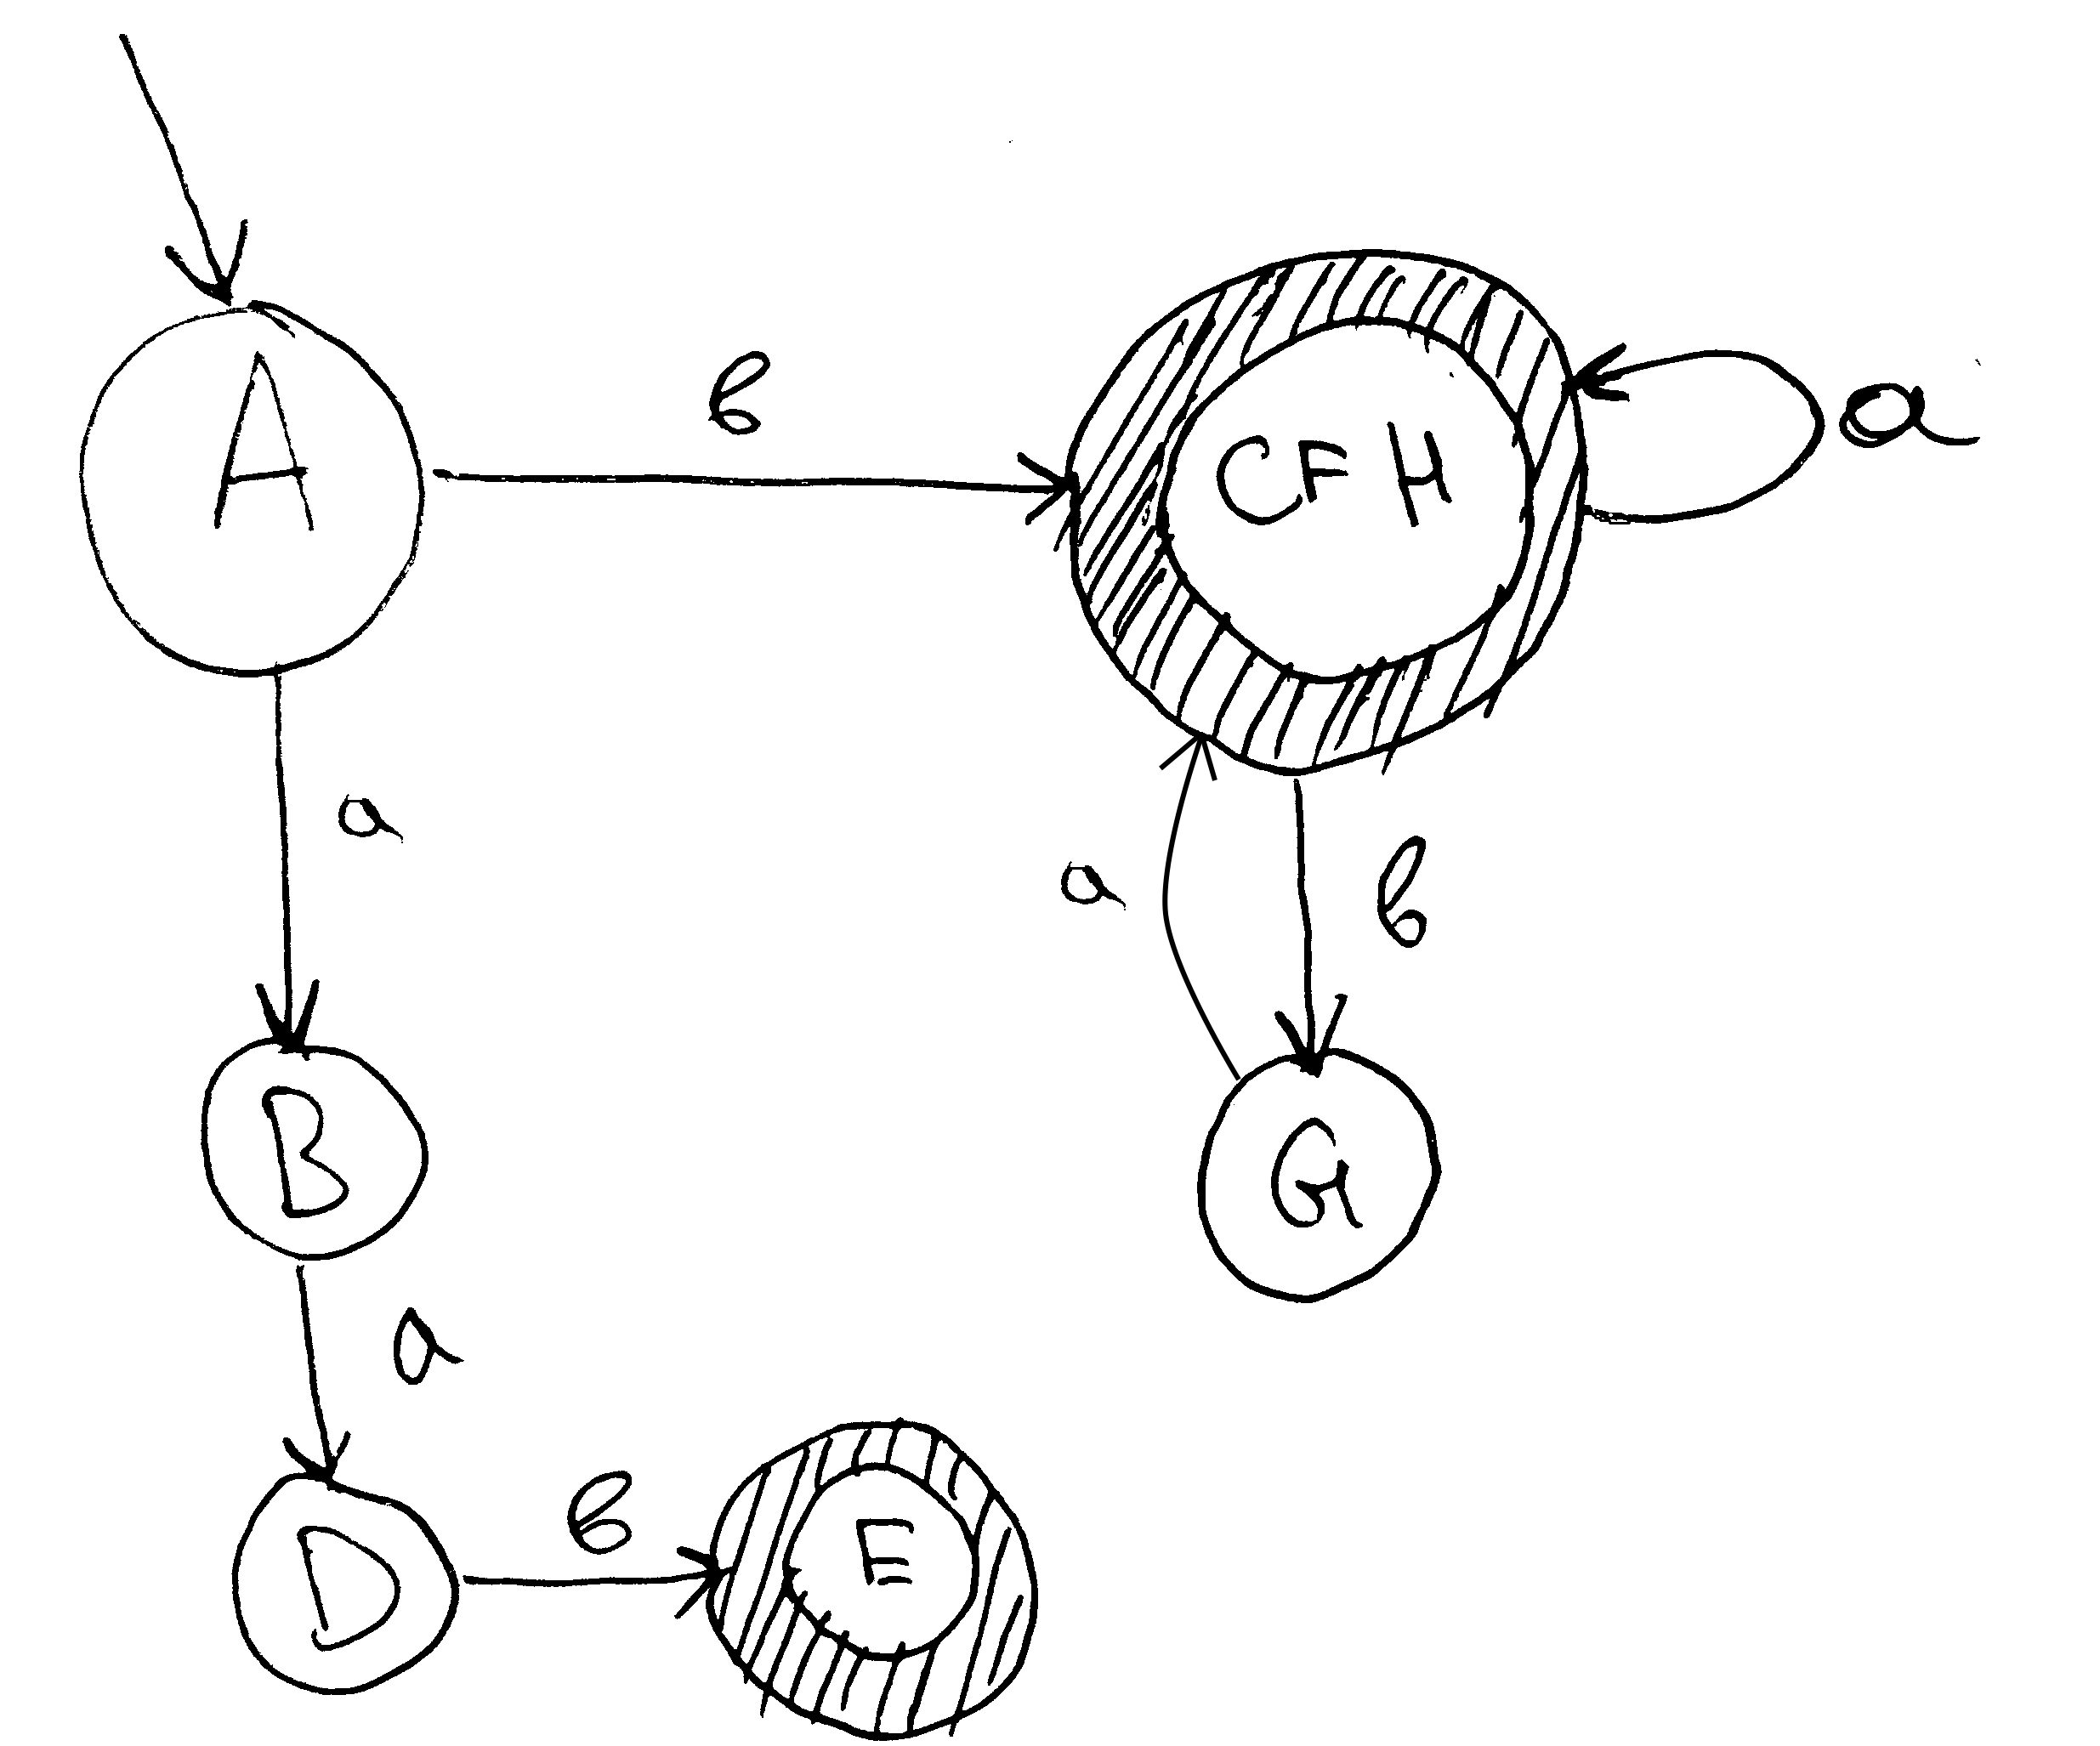
\includegraphics[scale=0.13]{data/pic4_2.png}
	\newpage
	\section{Почему это работает}
	На мой взгляд сам алгоритм говорит сам за себя, но чуть громче он будет говорить на фоне вот
	такого автомата:\\\\
	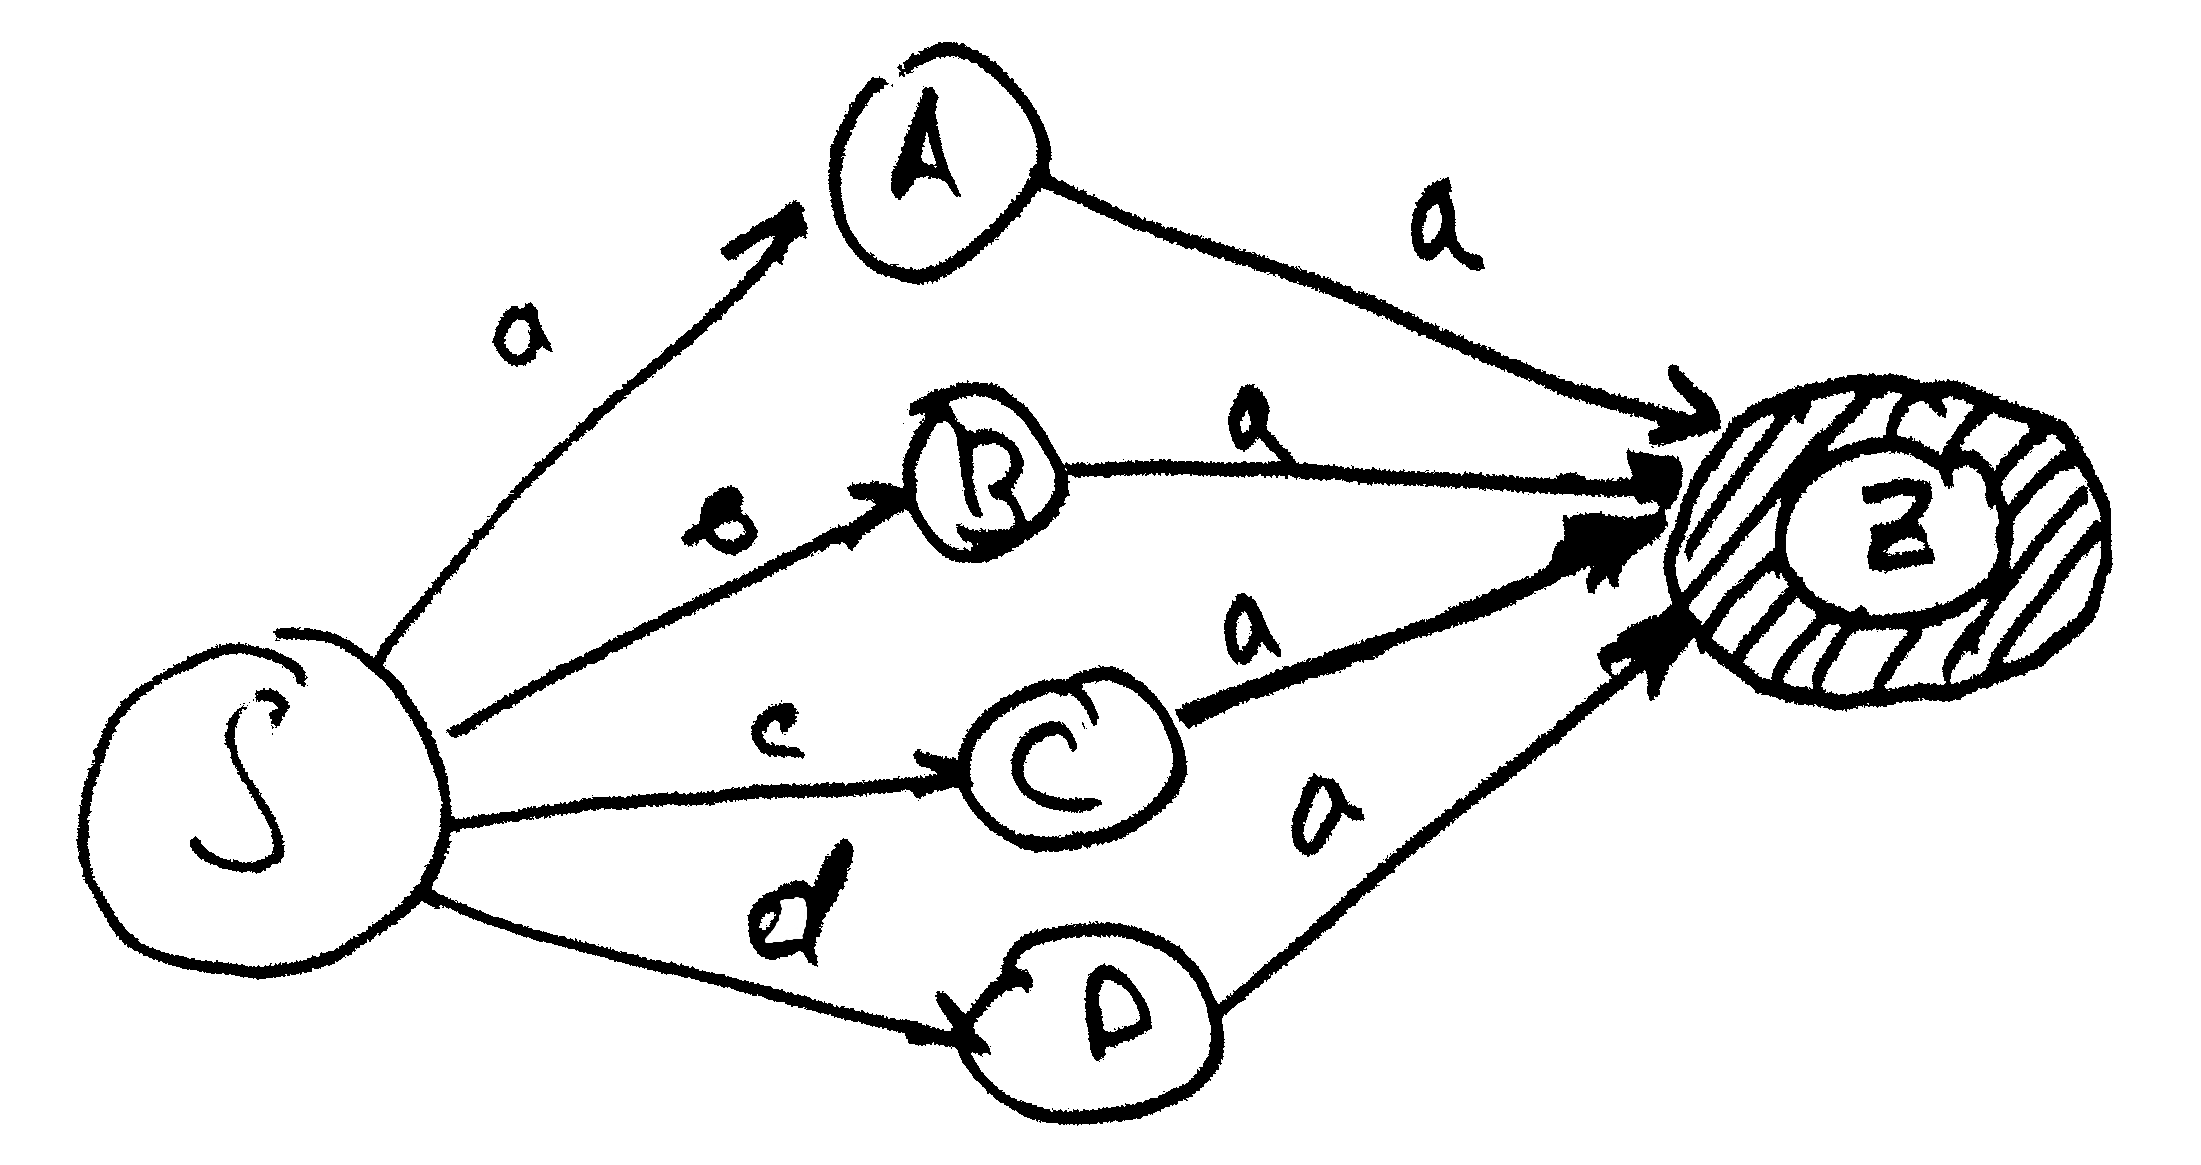
\includegraphics[scale=0.14]{data/pic4_3.png}
	\newpage
	\chapter{Отрицание, пересечение и объединение автоматов}
	Отрицание автомата $AVT$ - такой автомат $\overline{AVT}$, который успешно обрабатывает
	любую цепочку, которую не обрабатывает $AVT$.\\\\
	Пересечение автоматов $AVT1$ и $AVT2$ - такой автомат $AVT3$, который успешно обрабатывает
	любую цепочку, которую успешно обрабатывает и $AVT1$, и $AVT2$.\\\\
	Объединение автоматов $AVT1$ и $AVT2$ - такой автомат $AVT3$, который успешно обрабатывает
	любую цепочку, которую успешно обрабатывает хотя бы один из $AVT1$, $AVT2$.\\\\
	Любопытный читатель может спросить: а на кой это вообще все надо?\\
	Ну во-первых, такое задание могут дать на экзамене.\\
	А во-вторых, такое задание могут дать на экзамене в скрытой форме: вас могут попросить
	построить автомат, который принимает слова данной грамматики, но только четной длины.\\
	Тогда можно построить 2 автомата: первый принимает слова данной грамматики, а второй - слова
	четной длины. После этого их можно пересечь и радоваться жизни.
	\section{Алгоритм}
	Все алгоритмы требуют наличия дополнения.
	\subsection{Отрицание}
	А тут все совсем просто.
	\chapter{Построение автомата по праволинейной грамматике}
	\chapter{Приведение КС-грамматики}
	\chapter{Построение LL(1)-анализатора}
	\chapter{Построение LR(1)-анализатора по КС-грамматике}
	
	
	
	
\end{document}
